\chapter[L'\gls{edition-numerique} statique]{L'\gls{edition-numerique} statique : une solution soutenable et complémentaire}

Face aux limites identifiées des interfaces traditionnelles de bases de données, l'\gls{edition-numerique} statique propose une approche radicalement différente de la valorisation des données patrimoniales. Plutôt que de donner accès à l'ensemble du corpus via un moteur de recherche universel, elle privilégie une approche éditoriale : sélection raisonnée de contenus, organisation thématique, contextualisation narrative, parcours de découverte balisés.

Ce chapitre explore cette alternative en trois temps, suivant une progression logique du concept à sa mise en œuvre concrète. Il établit d'abord les fondements théoriques qui légitiment l'approche éditoriale statique : les principes d'éditorialisation adaptés au patrimoine musical baroque, les avantages techniques et économiques de l'architecture statique, et les enjeux environnementaux qui orientent vers des solutions de sobriété numérique. Ces fondements théoriques dessinent un cadre conceptuel qui guide les choix méthodologiques et techniques.

La méthodologie de transformation constitue le second volet de cette recherche. Elle détaille la conception d'un outil Python permettant l'éditorialisation collaborative des contenus, l'analyse des critères de sélection du corpus d'étude, et l'architecture de transformation \gls{xml}/\gls{xslt} qui automatise la génération des contenus web. Cette approche méthodologique traduit les principes théoriques en processus opérationnels reproductibles.

Enfin, la mise en œuvre technique examine concrètement la construction du site web généré : l'organisation des pages et des moyens de navigation, les stratégies de construction des notices individuelles, et les mécanismes complexes de récupération des relations entre entités musicologiques. Cette analyse technique révèle comment les choix de \glslink{mediationculturelle}{médiation} \glslink{algorithmie}{algorithmique} façonnent l'expérience utilisateur finale.

L'expérimentation pratique menée sur un corpus de quatorze projets issus de \textit{Philidor~4} permet d'explorer concrètement les potentialités et les limites de cette approche. Elle révèle notamment comment la transformation de données structurées en contenus web nécessite des choix éditoriaux constants : quelles données retenir ? comment les organiser ? quelle logique de navigation privilégier ? Cette réflexion sur la soutenabilité technique et environnementale ouvre des perspectives nouvelles pour la valorisation des données patrimoniales, questionnant les modèles dominants d'interfaces dynamiques et de bases de données en ligne.

\section[Du moteur de recherche à l'édition thématique]{Du moteur de recherche à l'édition thématique : changement de paradigme}

L'adoption d'une approche éditoriale statique pour la valorisation des données patrimoniales musicales nécessite d'établir ses fondements conceptuels et techniques. Cette démarche s'appuie sur trois piliers théoriques complémentaires qui justifient et orientent les choix méthodologiques : d'abord, les principes d'\gls{editorialisation-num} qui transforment la logique de consultation des bases de données ; ensuite, les avantages structurels de l'architecture statique en termes de performance et de sécurité ; enfin, les considérations environnementales qui s'imposent désormais dans les stratégies numériques institutionnelles. Ces trois dimensions convergent vers une alternative durable aux interfaces dynamiques traditionnelles.

\subsection{Principes d'éditorialisation et de contextualisation}

L'appréhension d'une base de données spécialisée dans la musique baroque représente un défi particulier pour les chercheurs, étudiants et mélomanes. Face à la complexité des sources historiques, la diversité des œuvres et la richesse contextuelle de cette période musicale, l'éditorialisation et la contextualisation émergent comme des stratégies essentielles pour rendre ces ressources numériques véritablement accessibles et exploitables.

\subsubsection{Définir l'\gls{editorialisation-num}}

L'\gls{editorialisation-num} est définie comme \textquote{toutes les actions destinées à structurer, rendre accessible et visible un contenu sur le web}\footcite{sinatraIntroduction2014}. Elle ne se limite pas à la simple mise en ligne de partitions, d'enregistrements ou d’informations sur un morceau, mais constitue un processus continu et ouvert de valorisation des ressources\footcite{mdupondVitaliRosatiMarcello20162020}.

Dans le contexte des bases de données musicales baroques, l'éditorialisation consiste à organiser, enrichir et présenter les contenus selon une logique qui facilite leur compréhension et leur appropriation par les usagers. Contrairement à l'édition traditionnelle, ce processus est évolutif et permet l'interaction continue avec les utilisateurs.

L'éditorialisation est définie comme un processus de réadaptation de contenus préexistants à l'environnement numérique interactif du web, les transformant pour de nouveaux contextes et publics\footcite{chartronEditionPublicationContenus2016}. Elle permet d'enrôler des ressources pour les intégrer dans une nouvelle publication\footcite{chartronEditorialisationQuoiParleton2020}.

Elle façonne la matière documentaire pour valoriser une collection patrimoniale ou créer de nouveaux documents\footcite{schopfelEditorialisationDonneesRecherche2020}. Ce processus inclut le marquage (identifiants, indexation, commentaires) et l'agrégation documentaire\footcite{schopfelEditorialisationDonneesRecherche2020}. Contrairement à l'édition traditionnelle qui fige le contenu, l'éditorialisation est donc un processus ouvert permettant l'enrichissement permanent des informations, souvent avec la participation des lecteurs\footcite{chartronEditionPublicationContenus2016}, qu'elle soit directe ou indirecte.

\subsubsection{La contextualisation : une nécessité pour la musique baroque}

La contextualisation revêt une importance cruciale pour la musique baroque en raison des spécificités historiques et culturelles de cette période. Les œuvres baroques s'inscrivent dans des contextes complexes impliquant les pratiques d'interprétation historiquement informées, l'ornementation spécifique, et les conventions stylistiques propres à chaque région européenne.

\begin{quotation}
	\textquote{\textit{L’exploration d’œuvres musicales, de représentations iconographiques ou encore de sources théoriques, dans le cadre d’une musicologie générale, ne peut faire l’impasse sur la prise en compte des contextes. Il s’agit d’une part de contextes de production et de réception et, de l’autre, de la signification contextuelle d’unités de sens au sein d’ensembles plus vastes (partitions, corpus iconographiques, écrits théoriques etc.).}}\footcite[consultée le 04/08/2025]{EpistemologieMusicologieNumerique}.
\end{quotation}

Cette approche est particulièrement pertinente pour les sources baroques, où l'improvisation et l'ornementation non écrites constituent des éléments essentiels de l'interprétation.

La contextualisation permet d'ancrer les œuvres musicales baroques dans leur environnement culturel et social. Elle facilite la compréhension des enjeux esthétiques et techniques spécifiques à cette période :

Il est possible d'évoquer le contexte sociopolitique avec le rôle des cours princières, des commandes ecclésiastiques ou encore du développement de l'opéra public. Il peut aussi être intéressant d'aborder le contexte esthétique avec l'affirmation de l'expressivité, le développement de la rhétorique musicale mais aussi l'émergence du système tonal\footcite{francois-sappeyChapitreIIAge2023}. Enfin, le contexte technique peut enrichir l'expérience utilisateur en abordant l'évolution des instruments, les pratiques d'ornementation et les conventions d'interprétation.

La contextualisation permet également de relier les œuvres aux sources documentaires contemporaines : traités théoriques, correspondances de compositeurs, témoignages d'époque. Cette approche enrichit considérablement la compréhension des œuvres en les replaçant dans leur contexte de création et de réception.

\subsubsection{Facilitation de l'accès et de l'appropriation}

L'éditorialisation facilite également la création de parcours thématiques qui guident l'utilisateur dans sa découverte. Ces parcours peuvent s'organiser autour de personnages importants, de genre musical, etc. L'éditorialisation vise à améliorer l'ergonomie des sites, rendre la navigation plus aisée et créer des liens plus efficaces entre les informations, ce qui était une faiblesse des systèmes plus anciens. Les liens dynamiques entre fiches (œuvres, biographiques, événements, bibliographies) facilitent la navigation.

L'éditorialisation et la contextualisation réduisent les obstacles à l'appropriation des contenus musicaux baroques. Elles permettent notamment une navigation intuitive adaptée aux différents niveaux d'expertise des utilisateurs et une présentation graduée des informations, du niveau introductif au niveau expert.

Ces approches permettent d'élargir l'\gls{accessibilite} des bases de données au-delà du seul public académique\footcite{FaciliterReperageAcces2014}. Les étudiants ont accès à un parcours structuré et à des ressources d'apprentissage contextuel. Les musiciens trouvent des informations pratiques sur les œuvres et l'interprétation historiquement informée. Enfin, les mélomanes ont accès à des présentations accessibles et engageantes des œuvres et compositeurs.

L'éditorialisation et la contextualisation constituent ainsi des stratégies complémentaires essentielles pour transformer les bases de données musicales baroques en véritables outils de connaissance et de découverte. En structurant l'accès aux ressources et en les ancrant dans leurs contextes historiques et culturels, elles facilitent l'appropriation de ce patrimoine musical complexe et riche, tout en ouvrant de nouvelles perspectives pour la recherche et la \gls{mediationculturelle}.

Cette approche éditoriale se concrétise par le développement d'un prototype d'édition statique appliqué aux données de \textit{Philidor~4}. Avant d'analyser les outils développés, il convient d'examiner les avantages techniques et écologiques qui ont motivé le choix de l'architecture statique.

\subsection{Avantages du statique : rapidité, résilience, coût}

L'architecture statique présente des avantages techniques et économiques substantiels qui la distinguent des solutions dynamiques traditionnelles. Ces bénéfices, particulièrement pertinents pour les institutions patrimoniales aux ressources souvent contraintes, touchent trois dimensions essentielles : la performance technique, la sécurité informatique et la viabilité économique.

\subsubsection{Performance et rapidité d'accès}

L'\gls{editionwebstatique} optimise significativement les performances d'affichage des contenus patrimoniaux par plusieurs mécanismes techniques convergents.

Le gain le plus immédiat réside dans la réduction des traitements côté serveur. Contrairement aux systèmes dynamiques qui construisent les pages à chaque requête utilisateur, le contenu statique est pré-généré, éliminant ainsi les opérations de calcul, les requêtes de base de données et les assemblages de templates au moment de la consultation\footcite{benzingLuwakContentManagement2006}. Cette architecture allège considérablement la charge computationnelle des serveurs, se traduisant par des temps de réponse nettement plus courts.

La légèreté structurelle des pages statiques constitue un second facteur d'optimisation. Les sites statiques présentent généralement des tailles de fichier réduites, diminuant la bande passante nécessaire au transfert des données et accélérant les temps de chargement\footcite{novaLowtechNumeriqueAux2020}. Cette économie de ressources bénéficie particulièrement aux utilisateurs disposant de connexions limitées ou d'appareils moins performants.

L'approche statique favorise également une conception épurée qui privilégie l'efficacité à l'ornementation. Une mise en page simplifiée, débarrassée d'éléments visuels superflus comme les fonds d'écran excessifs, contribue directement à l'optimisation des temps d'affichage. Cette philosophie minimaliste vise à fournir juste assez d'informations pour une expérience utilisateur positive, alignant ainsi performance technique et qualité éditoriale.

Enfin, cette optimisation technique améliore l'\gls{accessibilite} numérique des ressources patrimoniales. Des sites plus légers et plus simples demeurent accessibles et se chargent rapidement sur des appareils plus anciens et via des réseaux de télécommunication moins performants, notamment les connexions 3G/4G\footcite{novaLowtechNumeriqueAux2020}. Cette caractéristique répond à l'objectif d'assurer que les ressources patrimoniales soient \textquote{librement et également accessibles à tous les utilisateurs}\footcite{otooleSustainableWebEcosystem2013}, et ce indépendamment des moyens techniques des usagers.

\subsubsection{Résilience et sécurité informatique}

L'architecture statique offre des garanties de sécurité supérieures aux systèmes dynamiques, aspect particulièrement critique pour les institutions patrimoniales qui conservent des données sensibles et doivent maintenir la continuité de service.

Le principal avantage sécuritaire réside dans la réduction drastique de la surface d'attaque. Les sites statiques n'utilisent généralement ni bases de données dynamiques ni scripts côté serveur pour générer du contenu. Pour gérer ces bases de données, le langage informatique utilisé est le plus souvent \gls{sql}. Il permet d'interagir avec des bases de données relationnelles, afin de créer, modifier, interroger et gérer les données qu’elles contiennent.

Cette simplicité architecturale élimine les vulnérabilités les plus communes du web, notamment les injections \gls{sql} et les attaques par \gls{xss}, qui représentent plus de 50~\% des vulnérabilités web\footcite{otooleSustainableWebEcosystem2013}.

Les attaques par injection \gls{sql} exploitent les failles dans le traitement des données utilisateur pour insérer du code malveillant dans les requêtes de base de données\footcite{clarke-saltSQLInjectionAttacks2012a}. En l'absence de vérification appropriée des entrées, les attaquants peuvent détourner les requêtes pour accéder à des informations sensibles, contourner l'authentification, ou modifier et exfiltrer des données confidentielles. Ces attaques s'avèrent d'autant plus dangereuses qu'elles exploitent les privilèges élevés des applications.

L'injection de scripts cible, quant à elle, le côté client, en insérant du code JavaScript malveillant dans les applications ou bases de données. Ce code, présenté à l'utilisateur à son insu, permet au navigateur d'exécuter des actions non prévues : vol de données, chargement de programmes malveillants depuis des serveurs externes\footcite{clarke-saltSQLInjectionAttacks2012a}. Ces techniques compromettent simultanément la sécurité des systèmes et la confidentialité des informations personnelles.

L'architecture statique neutralise ces menaces en servant les fichiers comme contenus \textquote{en lecture seule} depuis le serveur, les rendant moins susceptibles d'altération ou de destruction par des injections de code malveillant.

La conception statique tend également à minimiser la collecte de données personnelles, n'intégrant généralement pas de formulaires complexes, de profils utilisateurs ou de cookies tiers de suivi\footcite{novaLowtechNumeriqueAux2020}. Cette sobriété fonctionnelle diminue drastiquement les risques de vol d'identité et de fraude financière, tout en simplifiant la conformité aux réglementations sur la protection des données.

Enfin, la simplicité et la transparence de l'architecture statique facilitent les audits de sécurité. Contrairement aux systèmes dynamiques et aux \glslink{algorithmie}{algorithmes} complexes souvent opaques et protégés par le secret commercial\footcite{richardDansBoiteNoire2018a}, les sites statiques peuvent être aisément inspectés pour détecter d'éventuelles vulnérabilités.

\subsubsection{Optimisation économique}

L'\gls{editionwebstatique} présente des avantages économiques substantiels, particulièrement pertinents pour les institutions patrimoniales confrontées à des contraintes budgétaires croissantes.

La réduction des coûts de développement et de maintenance constitue le premier bénéfice économique. L'architecture simple des sites statiques se traduit par un code moins complexe, réduisant les besoins en développement spécialisé et en maintenance technique. Cette simplification diminue les coûts liés aux licences logicielles propriétaires et au personnel hautement qualifié nécessaire à la gestion de systèmes complexes.

L'optimisation des coûts d'hébergement représente un second avantage économique significatif. Les faibles exigences en ressources serveur des sites statiques permettent des solutions d'hébergement plus abordables. L'administration d'un serveur pour des applications dynamiques complexes s'avère technique et coûteuse\footcite{otooleSustainableWebEcosystem2013}, tandis que les sites statiques peuvent être hébergés sur des infrastructures simplifiées, voire bénéficier de solutions d'hébergement gratuit pour les projets d'envergure modeste.

La flexibilité architecturale des solutions statiques réduit également les coûts de refactorisation. Les projets dynamiques complexes peuvent engendrer des coûts de restructuration importants, particulièrement lorsqu'ils impliquent des équipes externes et des modifications itératives\footcite{gantierRetroingenierieWebdocumentaireFind2020}. La simplicité des sites statiques permet des changements plus flexibles et potentiellement moins coûteux, facilitant l'évolution des projets selon les besoins institutionnels.

Ces avantages économiques s'avèrent particulièrement stratégiques pour les institutions patrimoniales, leur permettant d'allouer leurs ressources limitées à la constitution et à l'enrichissement de leurs collections plutôt qu'à la maintenance d'infrastructures techniques complexes.

D'autre part, les avantages techniques et économiques de l'approche statique trouvent un prolongement naturel dans les considérations environnementales contemporaines. L'architecture statique s'inscrit en effet dans une démarche d'éco-conception qui répond aux enjeux environnementaux croissants du secteur numérique, questionnant les modèles énergétivores des solutions dynamiques traditionnelles.

\subsection{Éco-conception et impact environnemental}

L'\gls{editionwebstatique} s'inscrit dans une démarche d'éco-conception qui répond aux enjeux environnementaux croissants du secteur numérique. Cette approche adopte les principes du \textquote{numérique low-tech}, qui vise à réduire l'empreinte environnementale des technologies de l'information et de la communication\footcite{novaLowtechNumeriqueAux2020}. Dans un contexte où le secteur numérique consomme plus de 10~\% de l'électricité mondiale et émet environ un milliard de tonnes de CO\textsubscript{2} par an\footcite{bihouixHighTechOuLowTech2022}, cette approche alternative mérite une attention particulière pour les institutions patrimoniales soucieuses de leur impact environnemental.

\subsubsection{Réduction de la consommation énergétique}

Le principal avantage environnemental des sites web statiques réside dans leur architecture simplifiée qui nécessite moins de traitements côté serveur. Contrairement aux systèmes dynamiques qui construisent les pages à chaque requête utilisateur, le contenu statique est pré-généré, ce qui diminue considérablement la charge computationnelle sur les serveurs\footcite{benzingLuwakContentManagement2006}. Cette réduction des opérations de traitement se traduit directement par une baisse de la consommation d'énergie des infrastructures d'hébergement\footcite{bihouixTransitionEnergetiquePeutelle2019}.

La diminution de la consommation énergétique des serveurs et du flux de données global contribue ainsi directement à la réduction des émissions de carbone du secteur numérique\footcite{novaLowtechNumeriqueAux2020}. Cette approche s'avère particulièrement pertinente pour les institutions publiques qui doivent intégrer les objectifs de transition écologique dans leurs stratégies numériques.

\subsubsection{Sobriété numérique et optimisation des ressources}

L'édition statique favorise naturellement la sobriété en ressources par la légèreté de ses productions. Les pages statiques présentent généralement des tailles de fichier réduites, ce qui diminue la bande passante nécessaire au transfert des données et accélère les temps de chargement\footcite{novaLowtechNumeriqueAux2020}. Cette optimisation technique répond aux exigences d'un design léger et d'une efficacité du code, composantes essentielles d'un écosystème web durable\footcite{otooleSustainableWebEcosystem2013}.

Les choix de conception inhérents à l'approche statique --- mise en page épurée, optimisation des images, limitation des interactions dynamiques --- influencent directement et positivement la consommation d'énergie des pages\footcite{otooleSustainableWebEcosystem2013}. Cette simplicité conceptuelle s'aligne avec l'objectif de concevoir des objets numériques simples, robustes, réparables et utilisant les ressources avec parcimonie\footcite{bihouixHighTechOuLowTech2022}.

\subsubsection{Concentration sur l'essentiel et lutte contre l'effet rebond}

L'édition statique encourage une démarche de \textquote{réduction des besoins à la source} et de \textquote{baisse de la demande}, plutôt que de simplement substituer l'offre énergétique\footcite{bihouixTransitionEnergetiquePeutelle2019}. 
Autrement dit, il ne s'agit pas seulement de remplacer les serveurs ou les centres de données par des infrastructures moins consommatrices, mais de questionner en amont la pertinence même des services et fonctionnalités proposés. 
Cette approche remet en question la nécessité de fonctionnalités excessives (par exemple, des animations, des vidéos en arrière-plan ou des options rarement utilisées par l’utilisateur) et de flux de données massifs. 
En effet, malgré les gains d'efficacité technologique (processeurs plus rapides, réseaux plus performants), ces améliorations sont souvent neutralisées par l'effet rebond, un phénomène bien documenté où les usages augmentent et entraînent une consommation globale de données toujours plus importante\footcite{bihouixHighTechOuLowTech2022}. 

Des initiatives concrètes illustrent cette orientation vers la sobriété numérique. 
Par exemple, le \emph{Low-tech Magazine} a optimisé son site web en réduisant le poids des images (en limitant leur résolution et leur nombre) et en utilisant des polices de base, ce qui diminue significativement le flux de données et donc la consommation d'énergie nécessaire à l’affichage du site\footcite{novaLowtechNumeriqueAux2020}. 
Dans le même esprit, des outils numériques \textit{low-consumption} comme \emph{txti} (un service qui permet de créer des blogs très légers en texte brut) ou encore des thèmes WordPress de très petite taille démontrent la faisabilité de cette approche. 
Ces solutions montrent qu’il est possible de concevoir des services utiles et accessibles tout en réduisant fortement l’empreinte énergétique du numérique\footcite{novaLowtechNumeriqueAux2020}.

\subsubsection{Simplification des infrastructures et réduction de la complexité}

L'architecture statique permet de s'affranchir de la dépendance aux infrastructures complexes caractéristiques des systèmes dynamiques. Les \gls{cms} traditionnels et leurs bases de données associées, tels que ceux utilisés historiquement par \textit{Philidor} (JLB-NET, \textit{eZ Publish}), se révèlent coûteux en ressources et en maintenance\footcite{otooleSustainableWebEcosystem2013}. Les problématiques techniques liées aux logiciels propriétaires et aux migrations mettent en évidence la complexité et la fragilité de ces solutions dynamiques.

Une conception low-tech privilégie au contraire une réduction de la complexité technologique\footcite{lebasApprochesLowtechInnovation2024}, favorisant la robustesse et la pérennité des systèmes. Cette simplification architectural présente des avantages non seulement environnementaux mais aussi économiques et techniques pour les institutions patrimoniales.

En définitive, l'\gls{editionwebstatique}, par sa priorité accordée à la simplicité, à l'efficacité des ressources et à la réduction de la charge computationnelle, s'inscrit pleinement dans la vision d'un écosystème web durable et écologique. Elle constitue une alternative concrète à la course effrénée vers des solutions high-tech toujours plus gourmandes en énergie et en ressources\footcite{bihouixTransitionEnergetiquePeutelle2019}, offrant aux institutions patrimoniales une voie de valorisation numérique compatible avec les impératifs de transition écologique. 

Ces fondements théoriques dessinent un cadre conceptuel cohérent qui guide la conception d'une méthodologie pratique. La mise en œuvre concrète de ces principes nécessite le développement d'outils spécialisés et la définition de processus de transformation adaptés aux spécificités des données musicologiques.

\section{Orientation méthodologique}

La concrétisation des principes éditoriaux statiques passe par la conception d'une méthodologie opérationnelle qui articule outils techniques et choix scientifiques. Cette approche méthodologique se déploie selon trois axes complémentaires : le développement d'un environnement logiciel permettant la contribution éditoriale, la sélection raisonnée d'un corpus d'expérimentation représentatif des enjeux de \textit{Philidor~4}, et la mise en place d'une architecture de transformation automatisée qui traduit les données structurées en contenus web éditorialisés. Cette méthodologie hybride vise à concilier rigueur scientifique et \gls{accessibilite} technique pour les contributeurs non spécialisés qui pourront générer une vitrine statique grâce à un environnement simple et graphique (cf. figure \ref{appli-accueil} et annexe \ref{xml_to_web_app}).

\begin{figure}[h]
	\caption{Accueil du logiciel} \label{appli-accueil}
	\centering
	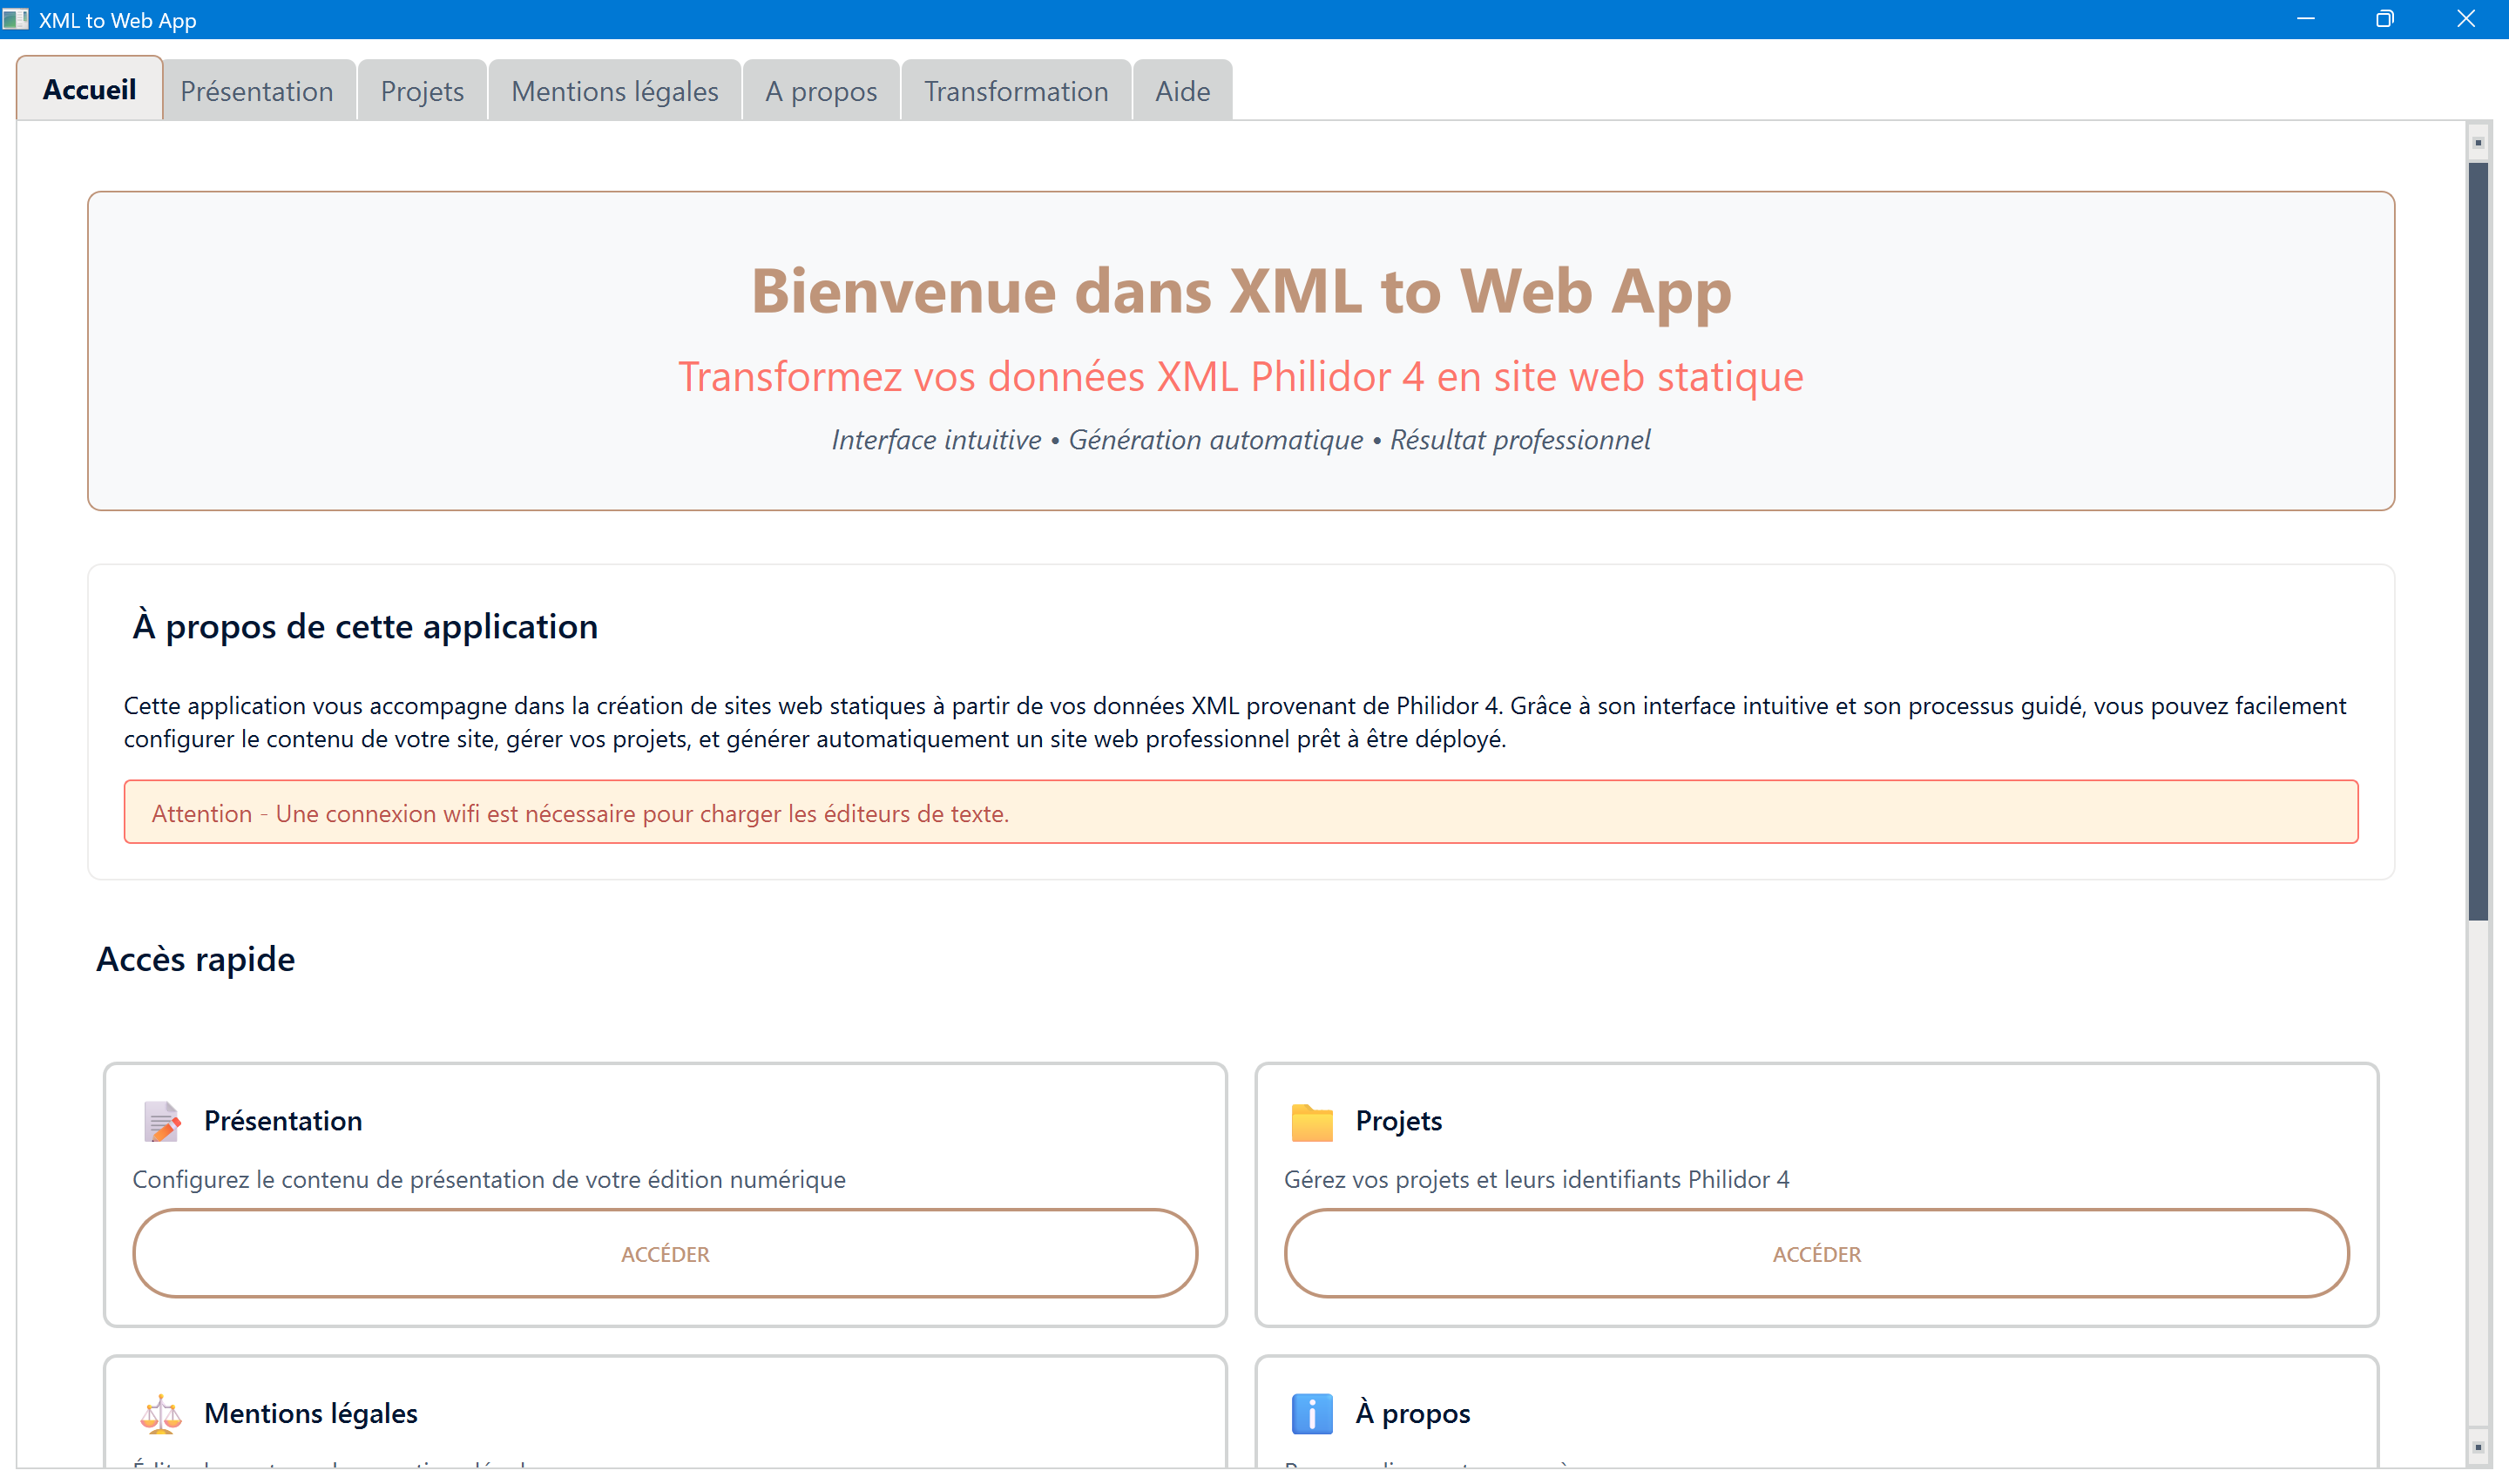
\includegraphics[width=\textwidth]{images/appli-accueil.png}
\end{figure}

\subsection{Outil d'édition collaborative et interface WYSIWYG}

Le développement d’un outil en Python pour générer des vitrines \gls{html} à partir d’extraits de la base \textit{Philidor~4} a pour but de permettre aux utilisateurs non techniques de contribuer à l’enrichissement éditorial des contenus.

\subsubsection{Une interface d'édition accessible}

L'originalité de cette approche réside dans la mise en place d'une interface d'édition \gls{wysiwyg}, signifiant littéralement \textquote{ce que vous voyez est ce que vous obtenez}, qui masque complètement la complexité technique sous-jacente aux utilisateurs non spécialisés. Le \textit{Dictionnaire encyclopédique du livre} donne la définition de \gls{wysiwyg} suivante :

\begin{quotation}
	\textquote{\textit{Se dit d’un mode d’affichage qui permet de voir à l’écran la représentation fidèle de ce qui sera imprimé.}}\footcite{foucheDictionnaireEncyclopediqueLivre}
\end{quotation}

Ce type d'interface apparaît pour la première fois en 1975 avec le logiciel \textquote{Bravo} conçu par Charles Simonyi pour Xerox Alto, mais c'est seulement dans les années 80 que naissent les traitements de texte populaires comme \textit{MacWrite} d'Apple (1984)\footcite{souchierChapitreNumeriqueEst2019}. L'affichage \gls{wysiwyg} apparait alors comme une innovation majeure. Il a été particulièrement apprécié par le grand public qui ne maîtrisait pas les affichages informatiques professionnels ni les configurations visuelles des textes édités\footcite{souchierChapitreNumeriqueEst2019}.

Intégrer ce type d'interface dans un outil programmé en Python permet aux chercheurs, bibliothécaires et documentalistes de contribuer directement au processus éditorial sans maîtriser les technologies \gls{xml} ou \gls{html}.

\subsubsection{Architecture modulaire de l'éditeur WYSIWYG}

L'architecture de l'éditeur repose sur une conception modulaire qui sépare clairement les responsabilités techniques et éditoriales. La classe abstraite \codeinline{python}{BaseEditorWidget} définit un cadre générique pour tous les types d'éditeurs, tandis que des implémentations spécialisées gèrent les différents contenus éditoriaux : présentation générale (cf. figure \ref{appli-onglet-presentation}), descriptions de projets, informations légales. Cette approche modulaire facilite l'extension du système et garantit la cohérence de l'interface utilisateur.

L'éditeur intègre un système de double visualisation (cf. figure \ref{appli-onglet-presentation}) qui permet aux utilisateurs de travailler selon deux modalités : un mode visuel utilisant TinyMCE comparable à un traitement de texte classique, et un mode code \gls{html} pour les utilisateurs plus techniques. Avec l'éditeur de texte riche \gls{wysiwyg}, l’utilisateur peut structurer son contenu, insérer des liens, souligner des termes ou ajouter des citations sans jamais quitter l’environnement visuel. Il n'a donc pas besoin d'avoir des connaissance en \gls{html} pour écrire ses contenus.

\begin{figure}[h]
	\caption{Onglet de modification de la présentation de l'édition} \label{appli-onglet-presentation}
	\centering
	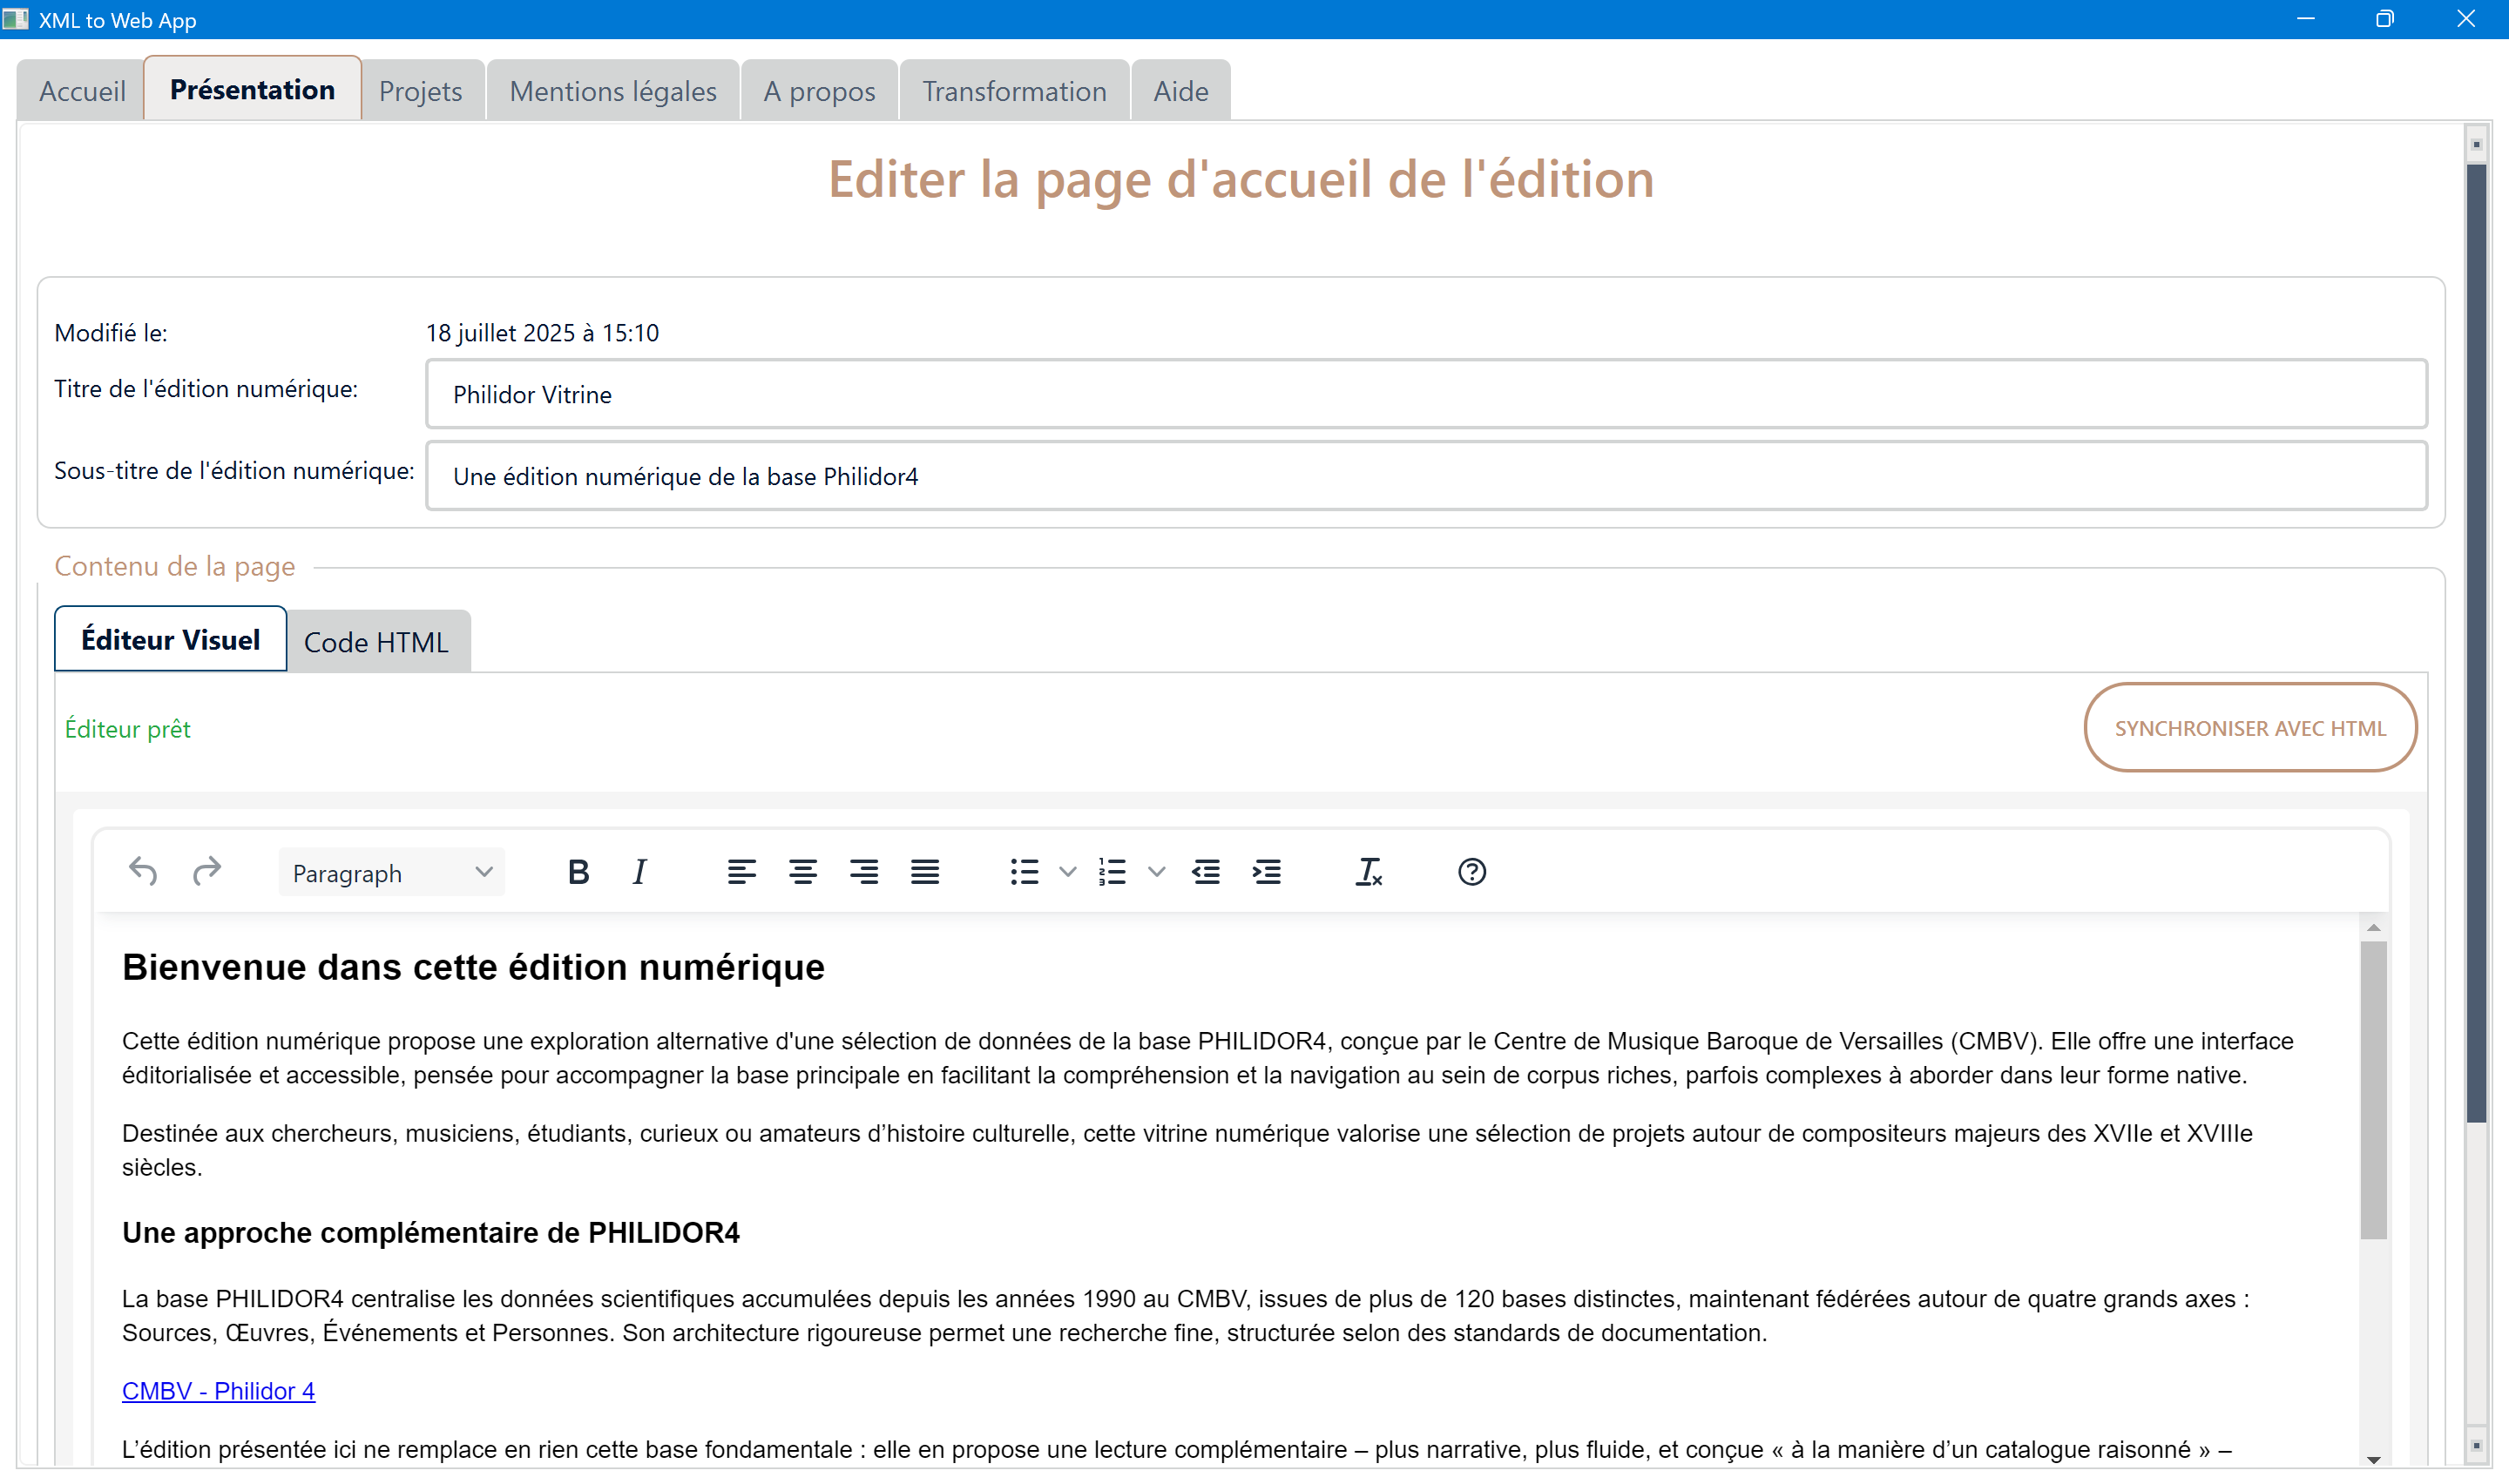
\includegraphics[width=\textwidth]{images/appli-onglet-presentation.png}
\end{figure}

La synchronisation automatique entre les deux modes évite les pertes de données et offre une flexibilité d'usage adaptée aux différents profils d'utilisateurs. Cette dualité constitue un compromis pertinent entre simplicité d'usage et contrôle précis du rendu final.

L'intégration de \codeinline{python}{QWebEngineView} avec TinyMCE représente un défi technique particulier en raison de la communication bidirectionnelle nécessaire entre l'environnement Python et le moteur JavaScript de l'éditeur. La classe \codeinline{python}{WysiwygEditor} gère cette complexité via un système de \textit{\glspl{callback}} asynchrones qui maintient la réactivité de l'interface tout en assurant la persistance automatique des modifications. Cette architecture évite les blocages d'interface et offre une expérience utilisateur fluide.

\subsubsection{Gestion des contenus et modélisation des données}

Le système de gestion des contenus s'appuie sur une modélisation orientée objet qui traduit chaque type de contenu éditorial en classe Python spécialisée. Par exemple, la classe \codeinline{python}{Presentation} encapsule toutes les métadonnées nécessaires à la page d'accueil : titre principal, sous-titre, contenu \gls{html} enrichi, heure de la dernière modification et métadonnées additionnelles. Cette approche garantit la cohérence des données tout en simplifiant leur manipulation programmatique.

La \gls{serialisation} \gls{xml} des contenus éditoriaux utilise une structure normalisée qui facilite leur réutilisation dans différents contextes. Chaque objet métier peut générer sa représentation \gls{xml} via des méthodes dédiées (\codeinline{python}{to_xml_element()}, \codeinline{python}{to_xml_string()}), tandis que la désérialisation inverse permet de reconstituer les objets à partir des fichiers sauvegardés. Cette bidirectionnalité assure la persistance des données éditoriales et leur portabilité entre différentes versions de l'outil.

La validation des contenus intervient à plusieurs niveaux : validation syntaxique des titres et sous-titres (longueur, caractères interdits), validation \gls{html} du contenu enrichi (balises autorisées, structure cohérente), et validation sémantique des métadonnées (cohérence des dates, intégrité des références). Cette approche préventive évite la génération de contenus mal formés et garantit la qualité du site web final.

L'outil implémente donc un \textit{\gls{workflow}} éditorial qui préserve l'intégrité des données. Chaque contenu éditorial dispose d'un historique automatique des modifications (création, dernière mise à jour) et d'un système de métadonnées extensible qui pourrait accueillir des informations de \textit{versioning} ou d'attribution.

L'interface de sauvegarde intègre une vérification automatique des modifications non sauvegardées, évitant les pertes de données accidentelles. Le système d'auto-sauvegarde périodique complète cette protection en préservant automatiquement les contenus en cours d'édition. Cette robustesse technique rassure les contributeurs non techniques et encourage l'adoption de l'outil dans des contextes institutionnels.

\subsection{Choix du corpus de données à éditer}

\subsubsection{Continuité éditoriale et contraintes du prototype}

Le corpus de quatorze projets retenus pour cette étude ne constitue pas un échantillon arbitraire. Ce choix s’explique notamment par les contraintes de temps liées à la réalisation de ce prototype. Une édition exhaustive de l’ensemble des données aurait dépassé le cadre imparti ; il a donc été nécessaire de cibler un corpus restreint mais représentatif. L’objectif n’est donc pas de clore un travail d’édition, mais de poser les bases d’une réflexion : d’une part en fournissant un socle réutilisable pour une édition complète future, d’autre part en expérimentant des modalités éditoriales susceptibles d’inspirer des améliorations de l’interface et de l’ergonomie de \textit{Philidor~4}.

\begin{figure}[h]
	\caption{Onglet présentant la liste des projets avec leurs métadonnées et l'aperçu de leur description} \label{appli-onglet-projets}
	\centering
	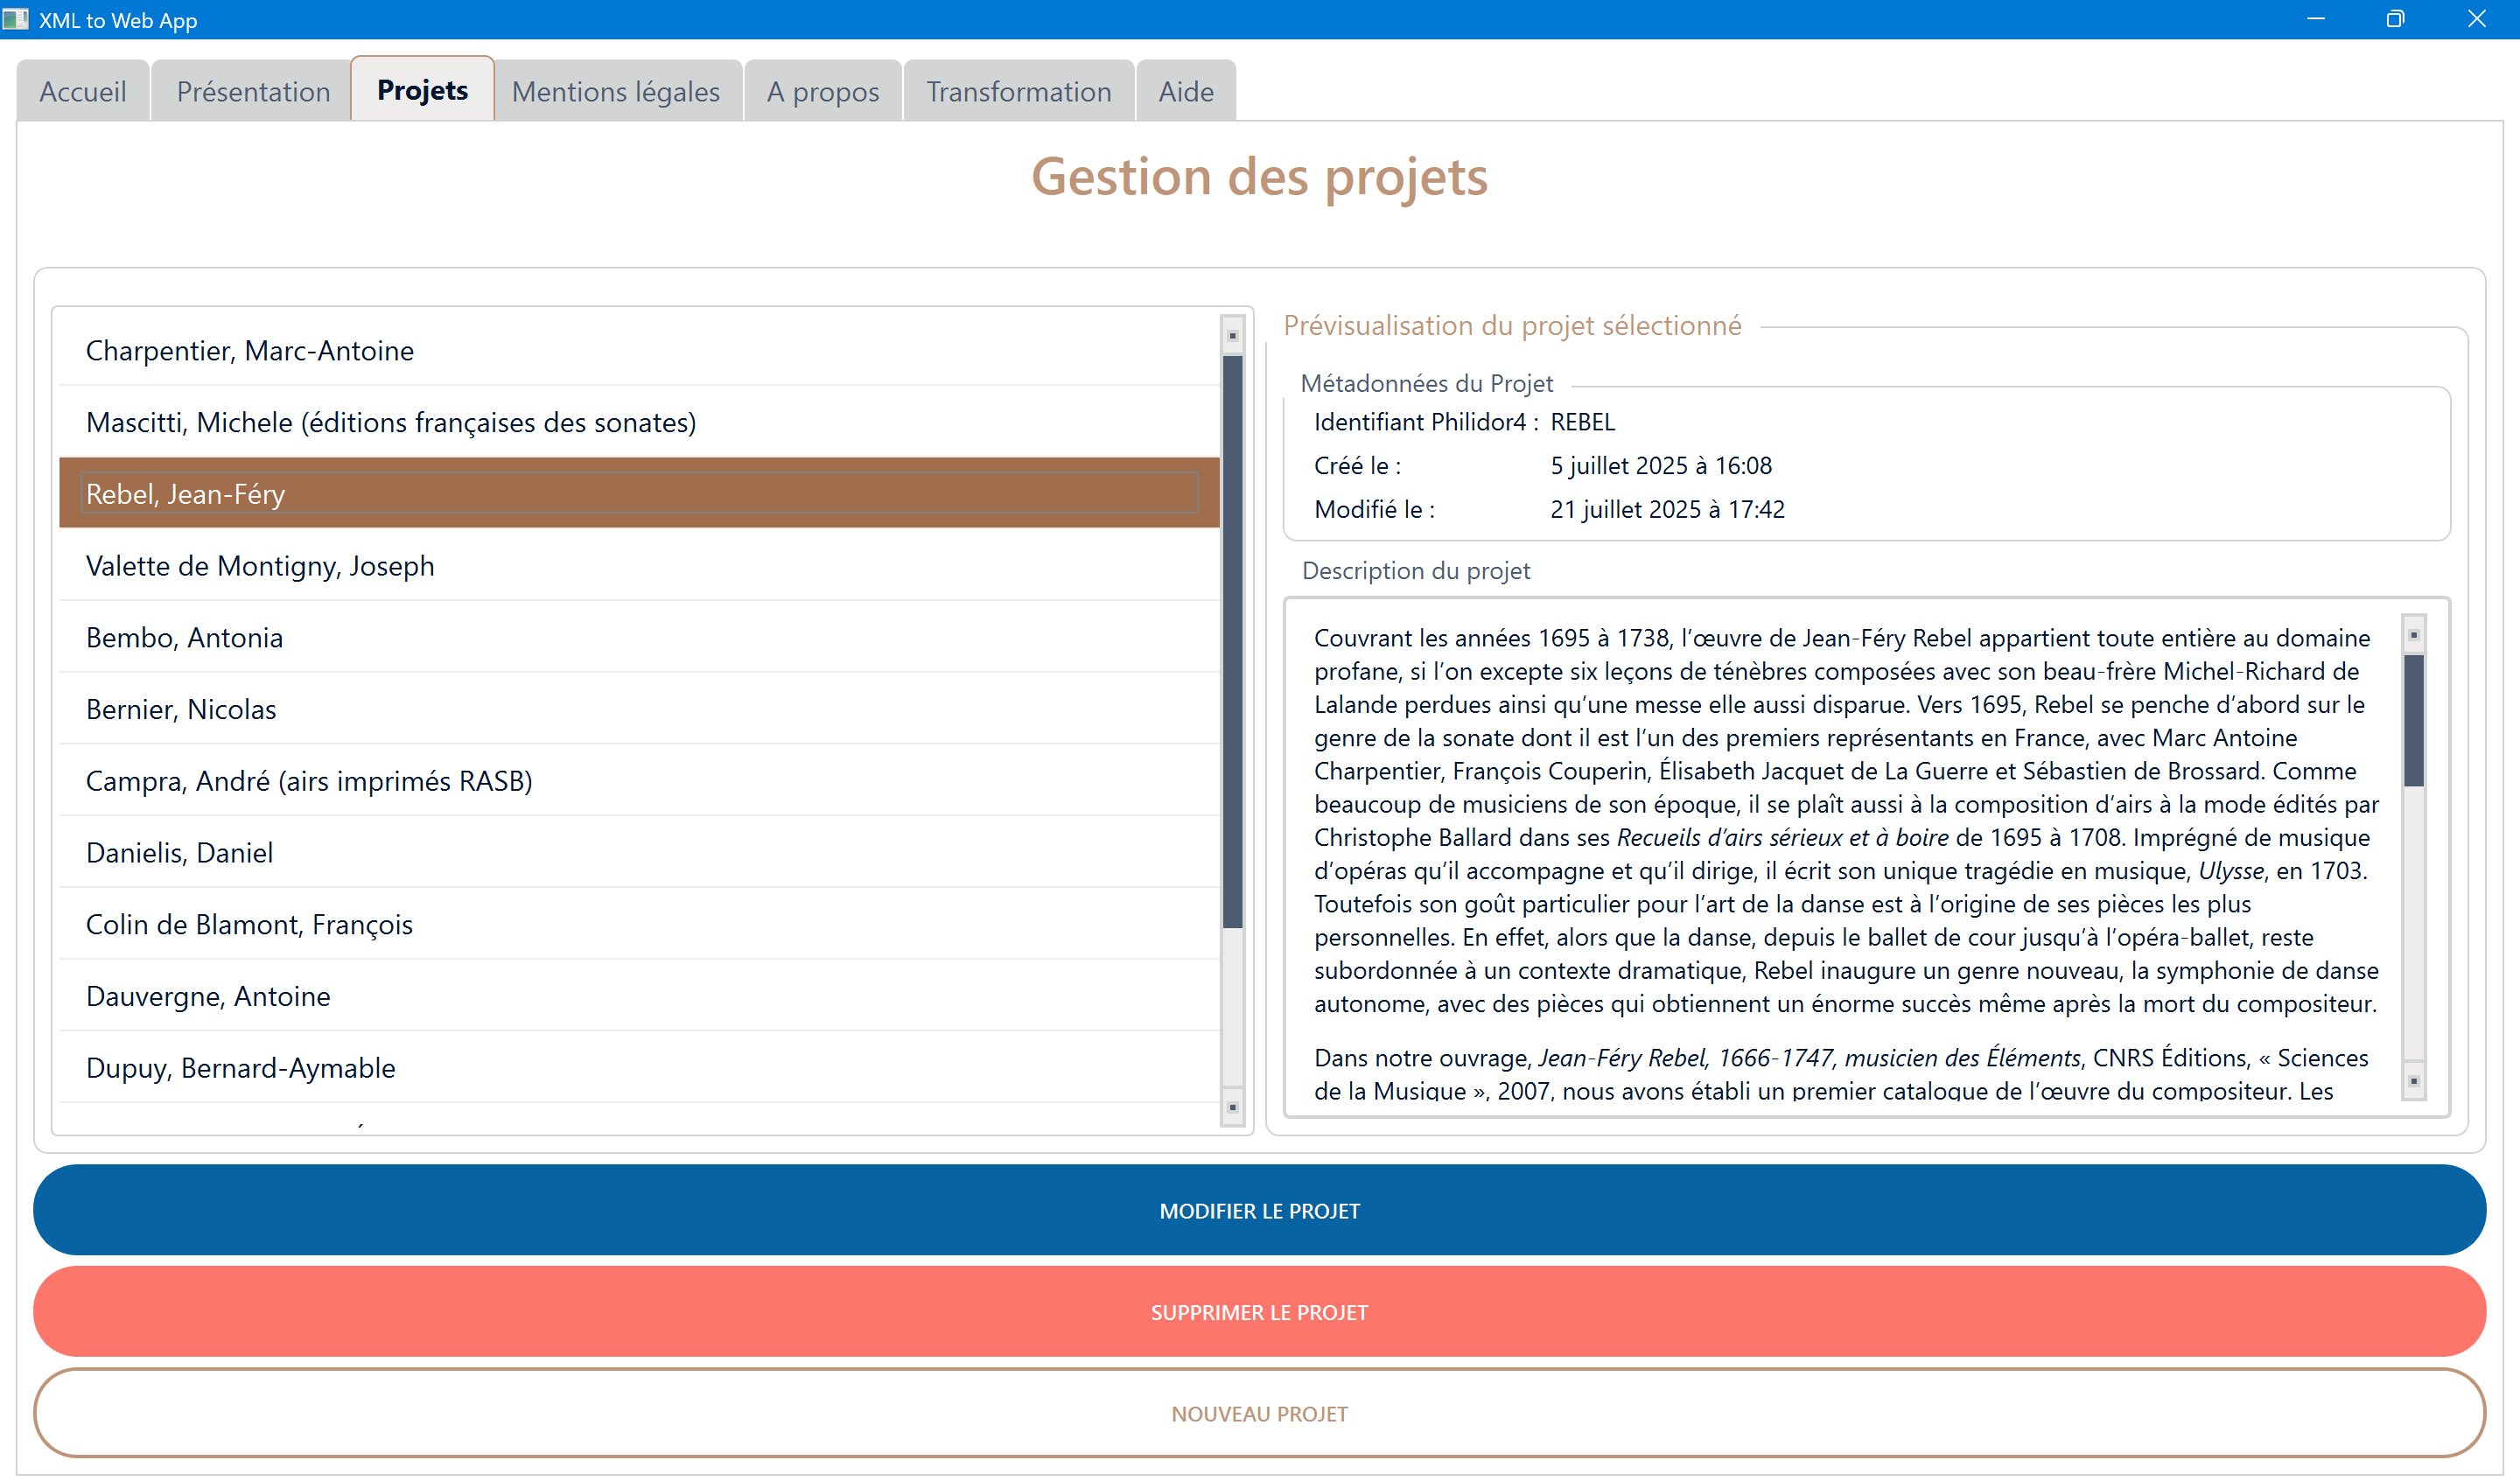
\includegraphics[width=\textwidth]{images/appli-onglet-projets.png}
\end{figure}

Les projets sélectionnés sont des projets déjà intégrés à \textit{Philidor III}, sous l'environnement \textit{eZ Publish} présenté au chapitre précédent, à l'exception d'un projet qui, bien qu'existant dans \textit{Philidor III}, n'a pas été retrouvé dans \textit{Philidor~4}. Leur sélection permet de disposer d'un socle de données qui avait déjà été jugé suffisamment propre et complet pour être édité et mis en ligne il y a plusieurs années. En effet, comme nous avons pu le voir, \textit{Philidor~4} contient des projets plus ou moins aboutis. Travailler dans un premier temps sur les données les plus complètes est d'une part plus simple pour la réalisation technique et plus agréable pour le public qui tombent ainsi sur des notices qui sont les plus exhaustives possibles. De plus, chacun de ces projets disposait d'une description dans \textit{Philidor III} ; ces dernières ont donc été reprises directement dans le prototype d'édition (cf. figure \ref{appli-onglet-projets}).

\subsubsection{La place des catalogues d’auteur dans \textit{Philidor~4}}

Les catalogues d’auteur représentent une part importante du contenu de la base \textit{Philidor~4}. Ils regroupent plusieurs milliers de notices et couvrent des compositeurs majeurs tels que Marc-Antoine Charpentier (2368 notices), Claude Le Jeune (630 notices), Bernard-Amable Dupuy (631 notices) ou encore Élisabeth Jacquet de La Guerre (50 notices). La prédominance numérique de ces catalogues illustre leur rôle central dans l’architecture documentaire de la base.

Sur le plan méthodologique, choisir d'éditer en priorité les catalogues d'œuvre semble être le plus pertinent. L’outil en \texttt{Python} décrit dans la sous-section précédente permet d’automatiser la génération de l’édition pour l’ensemble des projets sélectionnés et éditorialisés par l'utilisateur. Grâce à l’uniformité des structures propres aux catalogues d’auteur, l'utilisateur de cet outil peut ajouter autant de catalogue d'auteur qu'il le souhaite (cf. figure \ref{appli-popup-projet}) et mettre à jour l'\gls{edition-numerique}. 
En effet, la feuille de style mise en place peut être appliquée de manière homogène à d’autres corpus similaires, permettant d’ajouter aisément de nouveaux catalogues sans nécessiter de réécriture complète.

\begin{figure}[h]
	\caption{Onglet pop-up pour l'ajout ou la modification d'un projet} \label{appli-popup-projet}
	\centering
	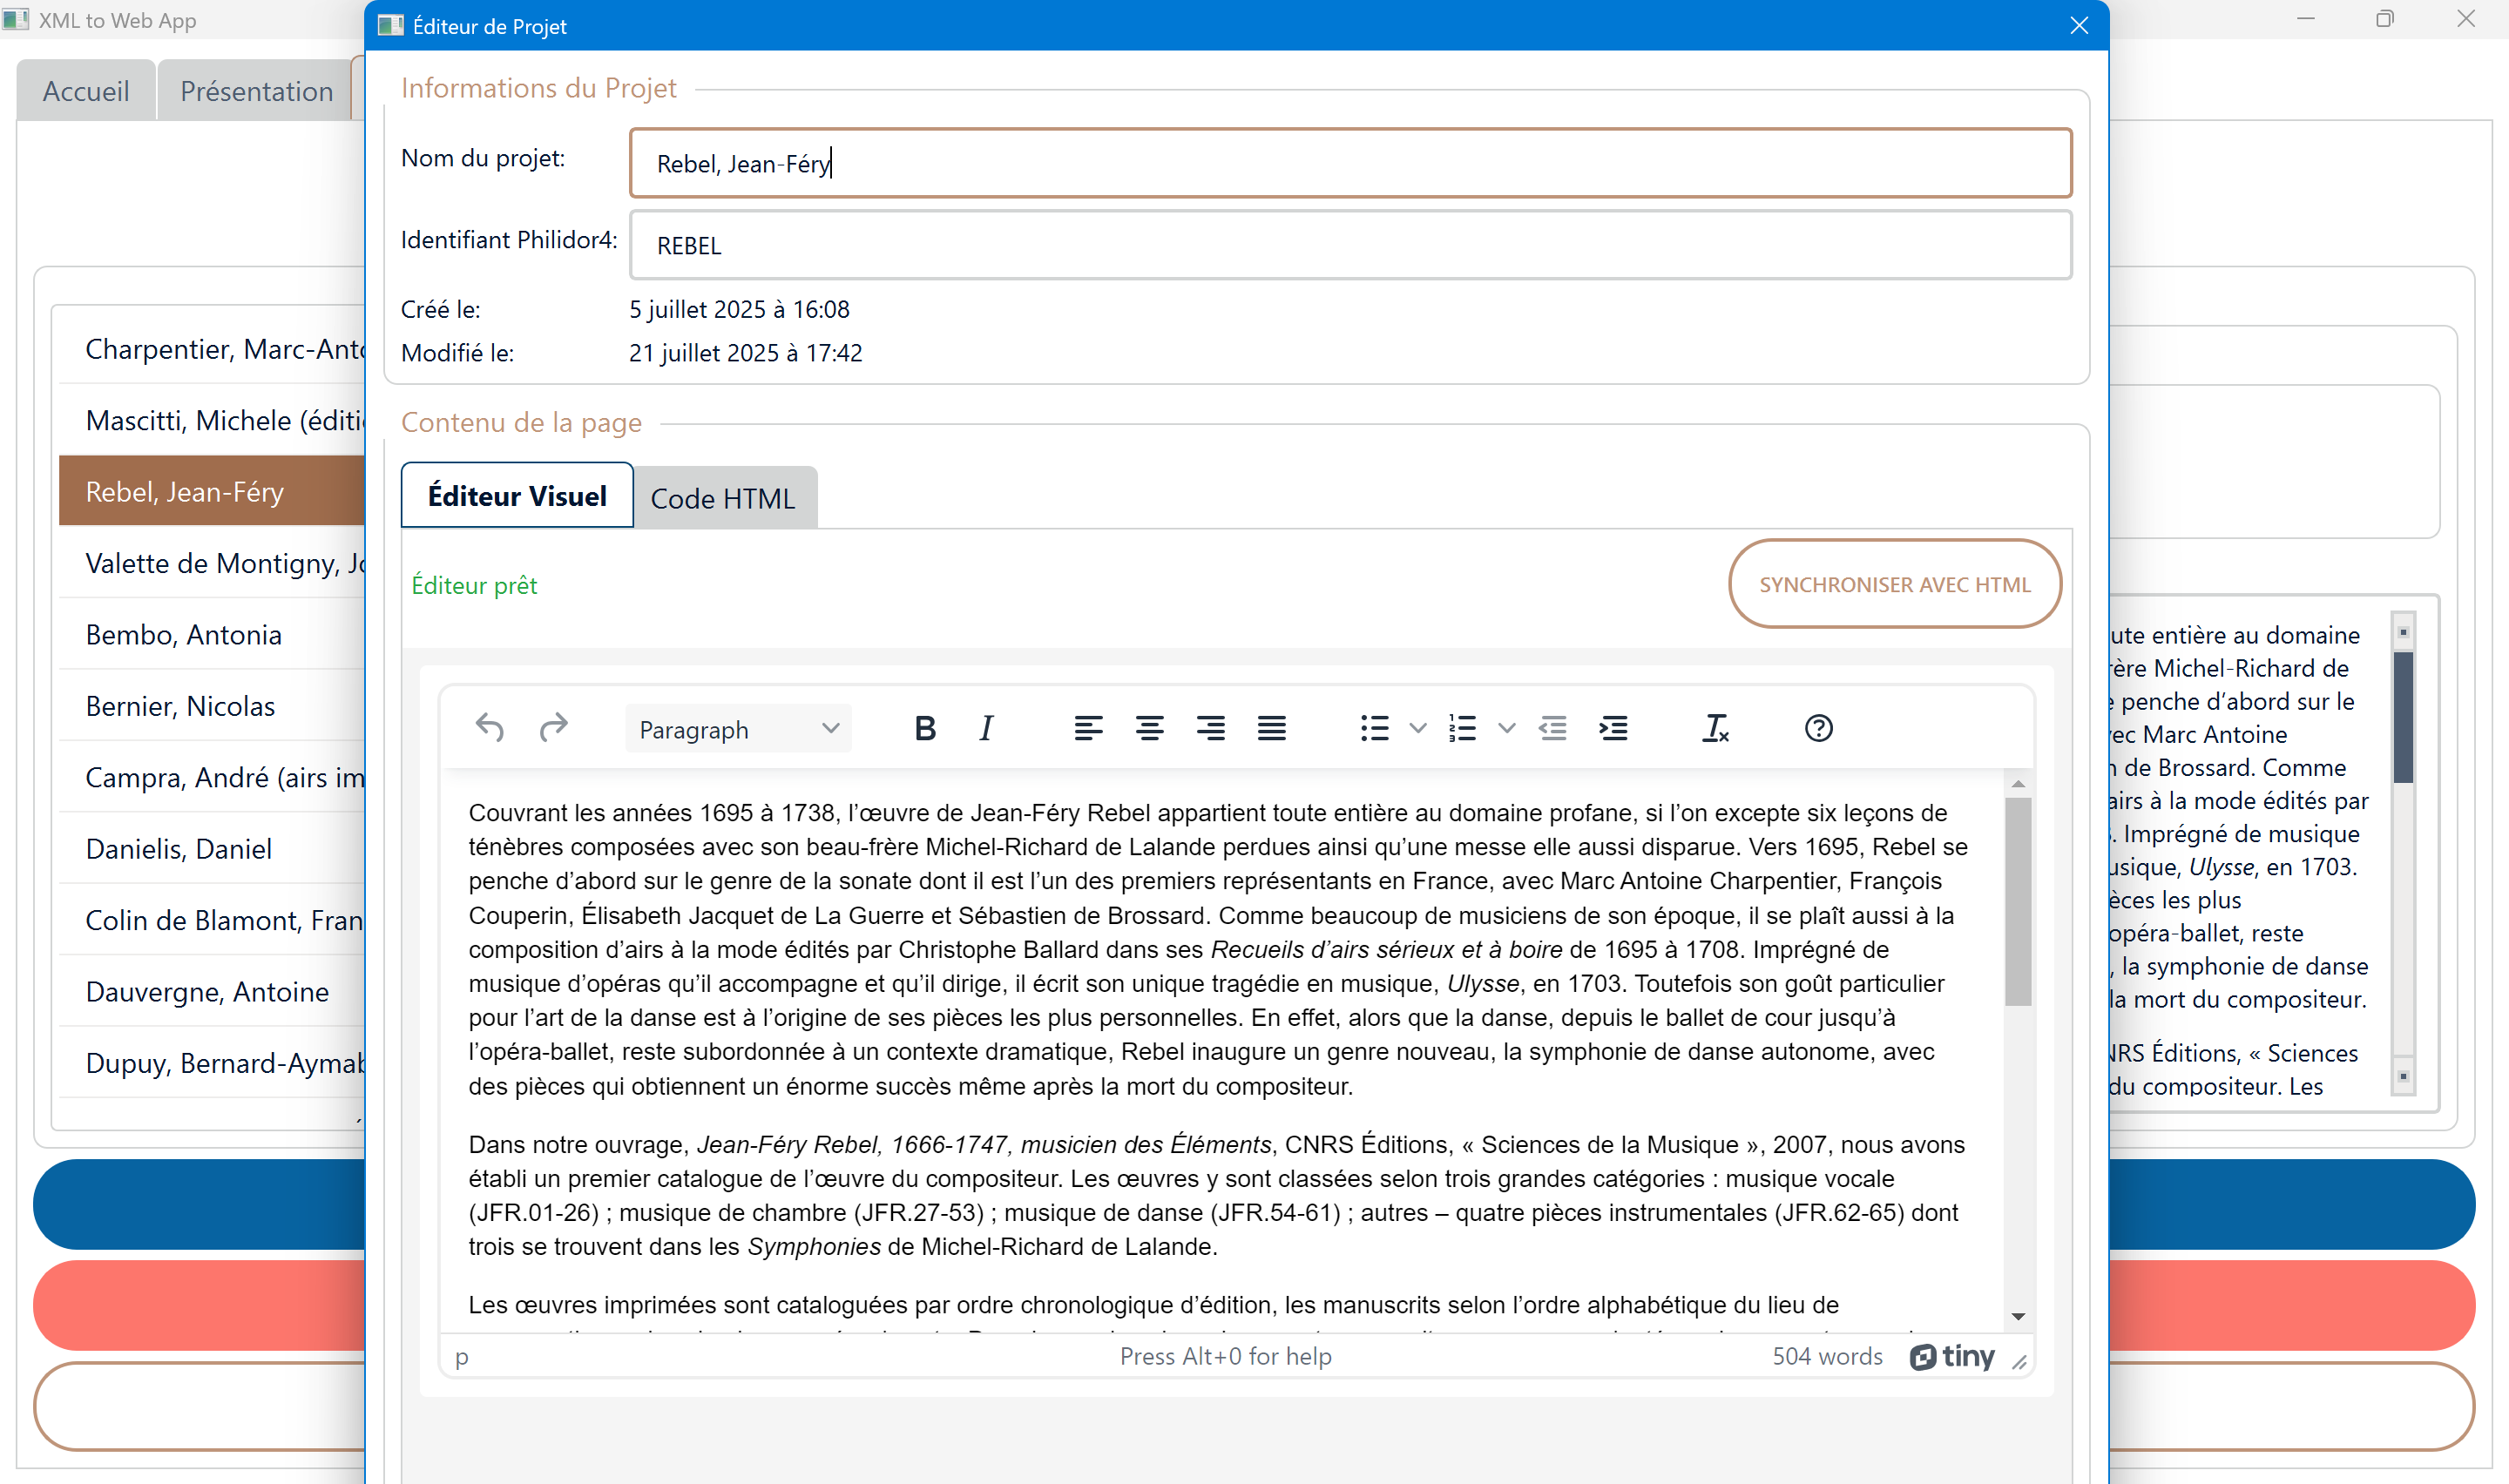
\includegraphics[width=\textwidth]{images/appli-popup-modif-projet.png}
\end{figure}

Ainsi, le choix de travailler prioritairement sur les catalogues d’auteur ne se justifie pas seulement par leur poids proportionnel dans \textit{Philidor~4}, mais aussi par leur valeur stratégique comme terrain d’expérimentation extensible pour les développements futurs de l’\gls{edition-numerique}.

\subsubsection{Diversité scientifique des corpus retenus}

Les projets sélectionnés couvrent une grande variété de situations documentaires et scientifiques. 
Certains se distinguent par l’ampleur de leur corpus (Charpentier, Le Jeune), véritables piliers de la musique française des XVI\textsuperscript{e} et XVII\textsuperscript{e} siècles. 
D’autres présentent une dimension intermédiaire (Bernier, Dupuy, Leclair), offrant un équilibre entre richesse documentaire et cohérence stylistique. 
Enfin, plusieurs ensembles plus restreints (Valette de Montigny, Bembo, Jacquet de La Guerre) apportent des perspectives précieuses sur la diversité des pratiques musicales et éditoriales.

\begin{longtable}{|l|c|c|}
\caption{Les quatorze projets retenus pour l’édition du prototype.} \\
\hline
\textbf{Projet} & \textbf{Œuvres} & \textbf{Sources} \\
\hline
\endfirsthead

\multicolumn{3}{c}%
{{\bfseries Suite du tableau précédent}} \\
\hline
\textbf{Projet} & \textbf{Œuvres} & \textbf{Sources} \\
\hline
\endhead

\hline \multicolumn{3}{r}{{Suite en page suivante}} \\
\endfoot

\hline
\endlastfoot

Antonia Bembo & 187 & 4 \\
\hline
Nicolas Bernier & 199 & 42 \\
\hline
André Campra (airs, RASB) & 77 & 78 \\
\hline
Marc-Antoine Charpentier & 2368 & -- \\
\hline
François Colin de Blamont & 104 & 10 \\
\hline
Daniel Danielis & 93 & 25 \\
\hline
Antoine Dauvergne & 86 & 5 \\
\hline
Bernard-Aymable Dupuy & 631 & 9 \\
\hline
Élisabeth Jacquet de La Guerre & 50 & 12 \\
\hline
Jean-Marie Leclair (imprimés) & 263 & 10 \\
\hline
Claude Le Jeune & 630 & 25 \\
\hline
Michele Mascitti & 114 & 10 \\
\hline
Jean-Féry Rebel & 63 & 17 \\
\hline
Joseph Valette de Montigny & 39 & 8 \\
\hline
\end{longtable}

Ainsi constitué, ce corpus offre un équilibre entre grands compositeurs, corpus moyens et ensembles restreints, tout en intégrant des dimensions stylistiques, géographiques, sociales et genrées. Il constitue un terrain d’expérimentation adapté aux contraintes d’un prototype, tout en ouvrant des perspectives pour des développements éditoriaux et techniques plus ambitieux. 

Cette méthodologie de transformation trouve sa concrétisation dans la mise en œuvre technique d'un site web statique. L'architecture logicielle ainsi définie doit alors se traduire en interfaces utilisateur fonctionnelles et en mécanismes de navigation adaptés aux pratiques de consultation musicologique.

Ce corpus de quatorze projets, constitué selon des critères de qualité et de représentativité, fournit la matière première de l'expérimentation éditoriale. Sa transformation en site web statique repose sur une architecture technique spécifique qui automatise le passage des données \gls{xml} vers les pages \gls{html} finales, nécessitant la mise en place d'un processus de transformation standardisé et reproductible.

\subsection{Architecture de transformation \gls{xml}/\gls{xslt}}

La transformation automatisée des données \textit{Philidor~4} en contenus web éditorialisés repose sur une architecture technique sophistiquée qui articule plusieurs composants logiciels spécialisés. L'utilisateur peut lancer la transformation directement depuis l'interface du logiciel. Pour lui, la partie technique est complètement invisible grâce à l'interface graphique (cf. figure \ref{appli-transformation}). Cette architecture de transformation constitue le cœur du processus de génération statique, traduisant les données structurées \gls{xml} en pages \gls{html} navigables tout en préservant la richesse informationnelle des notices musicologiques. L'analyse de cette architecture révèle les choix d'implémentation qui conditionnent à la fois la fidélité de la restitution des données et l'efficacité du processus de génération.

\begin{figure}[h]
	\caption{Onglet pour lancer la transformation et le téléchargement du résultat} \label{appli-transformation}
	\centering
	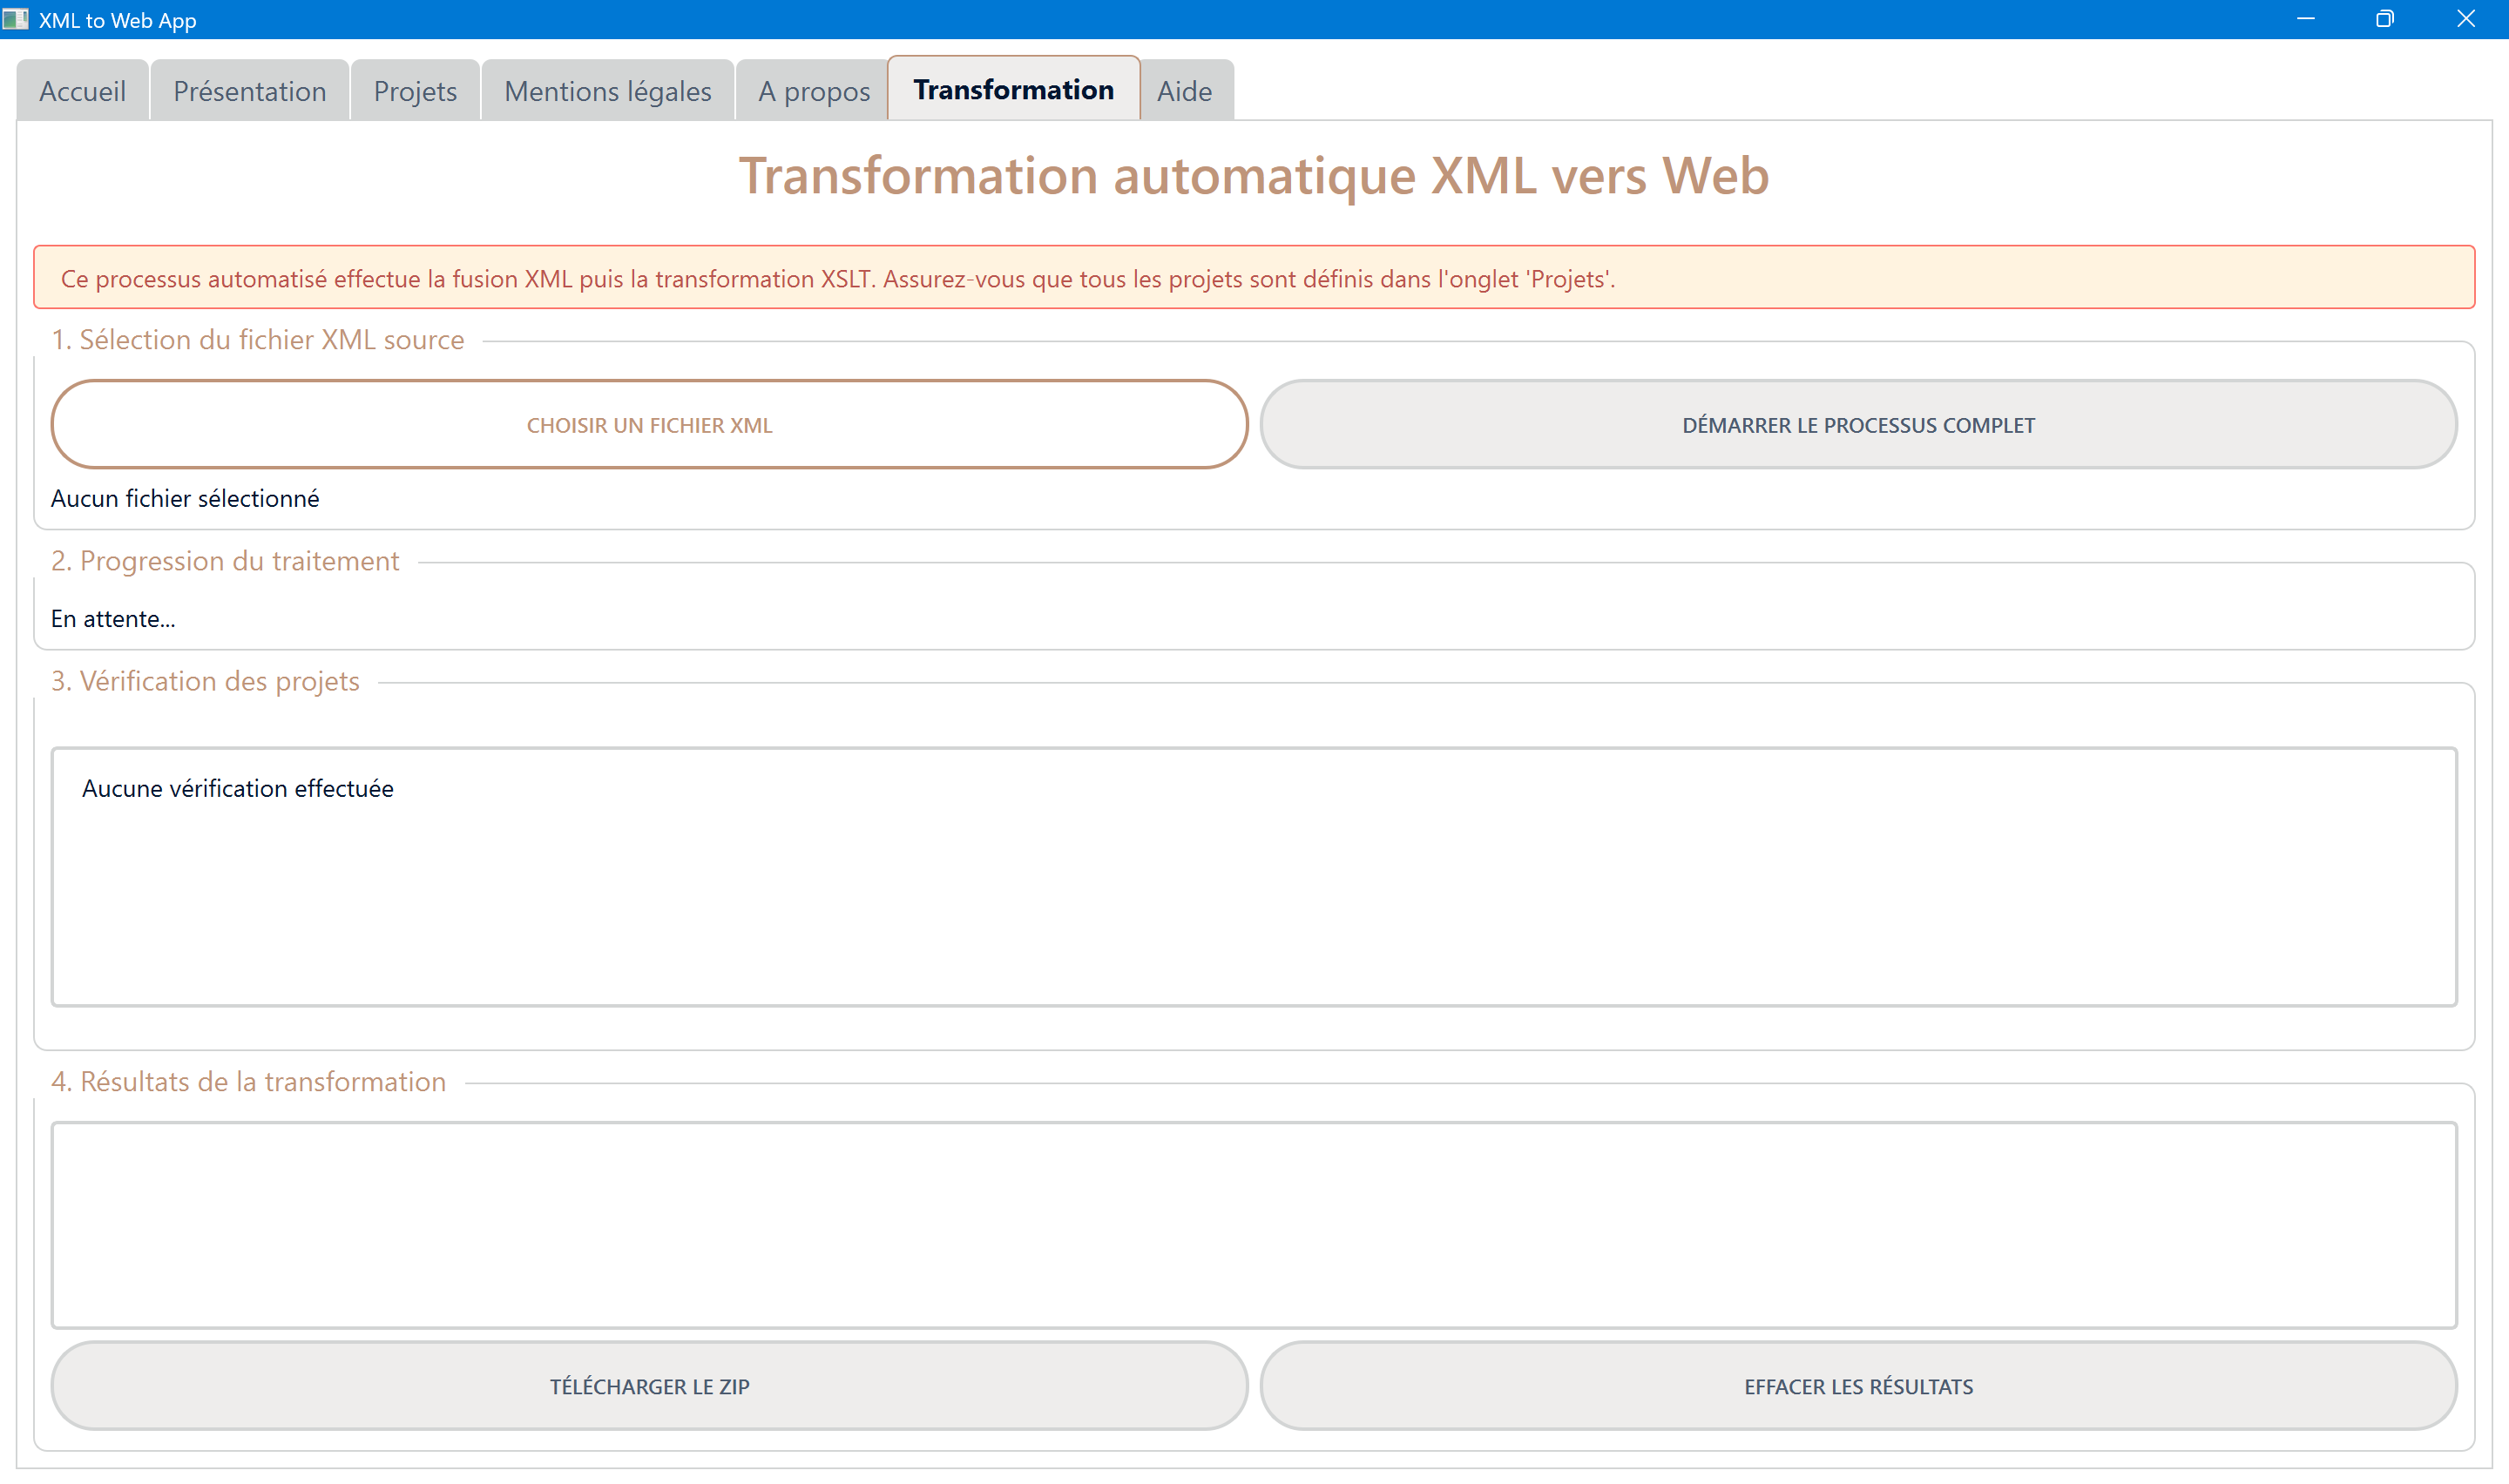
\includegraphics[width=\textwidth]{images/appli-onglet-transformation.png}
\end{figure}

\subsubsection{Moteur de transformation : architecture modulaire et flux de traitement}

L'architecture de transformation s'organise autour d'un moteur principal \codeinline{python}{XSLTTransformationEngine} qui orchestre l'ensemble du processus de conversion. Cette approche modulaire sépare clairement les responsabilités : gestion des fichiers temporaires, configuration des processeurs \gls{xslt}, pilotage des transformations et consolidation des résultats. Le moteur utilise la bibliothèque \textit{Saxon-CE} via l'interface Python \codeinline{python}{saxonche}, garantissant une compatibilité maximale avec les spécifications \gls{xslt} 3.0 et une robustesse éprouvée pour le traitement de documents \gls{xml} complexes.

La gestion des espaces de travail temporaires constitue un aspect crucial de l'architecture. Chaque transformation génère un identifiant unique (\gls{uuid}) qui structure l'organisation des fichiers intermédiaires et finaux dans des répertoires dédiés. Cette approche isole les transformations simultanées et facilite le débogage en cas d'erreur, tout en permettant un nettoyage automatique des ressources temporaires. L'organisation hiérarchique des répertoires de sortie \codeinline{text}{output/}, \codeinline{text}{output/statics/} reflète directement la structure du site web final, simplifiant l'assemblage des ressources.

Le processus de transformation intègre également un système de post-traitement automatique des entités \gls{html} encodées. Les données extraites de \textit{Philidor~4} contiennent fréquemment des caractères spéciaux doublement encodés \codeinline{text}{\&amp;#xE9;} pour \textquote{é}, nécessitant un décodage en cascade pour restaurer l'affichage correct des caractères accentués. Cette correction automatique évite les manipulations manuelles fastidieuses et garantit l'homogénéité de l'encodage dans les pages générées.

\subsubsection{Workflow de préparation et de consolidation des données}

L'architecture de transformation précède la phase \gls{html} proprement dite par un \textit{\gls{workflow}} complexe de préparation et de consolidation des données \gls{xml}. Le processeur \gls{xslt} \codeinline{python}{XMLProcessor} assume cette responsabilité critique en orchestrant plusieurs opérations de nettoyage, validation et fusion qui conditionnent la qualité de la transformation finale.

La phase de nettoyage \gls{xml} révèle la complexité inhérente au traitement de données patrimoniales hétérogènes. L'implémentation traite spécifiquement les anomalies structurelles récurrentes : balises \codeinline{xml}{<Anonyme>} non conformes, éléments vides redondants, caractères spéciaux mal échappés. Le nettoyage applique également une stratégie de suppression sélective des balises commençant par une majuscule\footnote{ces dernière étant des noms de personnes non normalisé comme vu dans le chapitre précédant}, tout en préservant les identifiants d'autorités normalisés (\glslink{viaf}{VIAF}, \gls{isni}, \glslink{idref}{IDREF}, \gls{bnf}). Cette approche pragmatique résout les incohérences de saisie tout en préservant l'intégrité des données critiques.

La consolidation des données opère ensuite une fusion structurée entre le fichier \gls{xml} principal et les contenus éditoriaux complémentaires. L'architecture génère un document \gls{xml} unifié \codeinline{xml}{<merged_data>} qui encapsule les données \textit{Philidor~4} dans une section dédiée \codeinline{xml}{<philidor4_data>} et y adjoint les contenus de présentation, informations légales et descriptions de projets. Cette approche évite les références externes multiples dans les transformations \gls{xslt} et simplifie considérablement la logique de traitement.

\subsubsection{Validation et vérification de cohérence}

L'architecture intègre un système de validation sophistiqué qui vérifie la cohérence entre les données de catalogage et les métadonnées de projets avant d'autoriser la transformation. Cette vérification cross-référentielle constitue une innovation importante qui prévient la génération de sites incomplets ou incohérents.

Le mécanisme de validation analyse les références de projets présentes dans les notices de catalogage et les confronte aux définitions de projets disponibles dans les contenus éditoriaux. L'implémentation utilise des opérations ensemblistes pour identifier précisément les projets manquants et générer des rapports d'erreur détaillés. Cette approche préventive évite la production de liens brisés ou de pages orphelines, garantissant l'intégrité fonctionnelle du site généré.

\subsubsection{Orchestration asynchrone et retour utilisateur}

L'architecture de transformation tire parti de la programmation asynchrone (Qt Threading) pour maintenir la réactivité de l'interface utilisateur durant les opérations potentiellement longues. Cette approche technique évite le blocage de l'interface et permet un retour d'information continu sur l'avancement des traitements.

L'implémentation définit des workers dédiés \codeinline{python}{TransformationWorker} qui exécutent les transformations \gls{xslt} en arrière-plan tout en émettant des signaux de progression vers l'interface principale. Cette architecture permet de traiter des corpus volumineux (plusieurs milliers de notices) sans dégradation de l'expérience utilisateur, aspect crucial pour l'adoption de l'outil dans des contextes institutionnels.

Le système de rapport automatique génère une documentation \gls{xml} détaillée de chaque transformation : fichiers sources, durée de traitement, nombre de pages générées, identifiant de session. Ces métadonnées facilitent le suivi des versions et le débogage des transformations complexes. La génération automatique d'archives ZIP autocontenantes simplifie la distribution et l'archivage des sites produits.

La génération de sites statiques autonomes simplifie drastiquement les problématiques de déploiement et de conservation. L'absence de dépendances runtime complexes facilite l'archivage à long terme et la migration entre environnements techniques. Cette autonomie technique renforce la pérennité des éditions produites et s'aligne avec les exigences de conservation numérique des institutions patrimoniales. L'interface graphique du logiciel permet à un utilisateur non technique de participer à l'éditorialisation. Il peut également générer l'ensemble du site web statique de l'édition en appyant sur un bouton sans se préoccuper du côté technique de la transformation. Un onglet aide (cf. figure \ref{appli-onglet-aide}) et des boîtes de dialogue sont disponible pour accompagner l'utilisateur dans son usage du logiciel.

\begin{figure}[h]
	\caption{Onglet d'aide} \label{appli-onglet-aide}
	\centering
	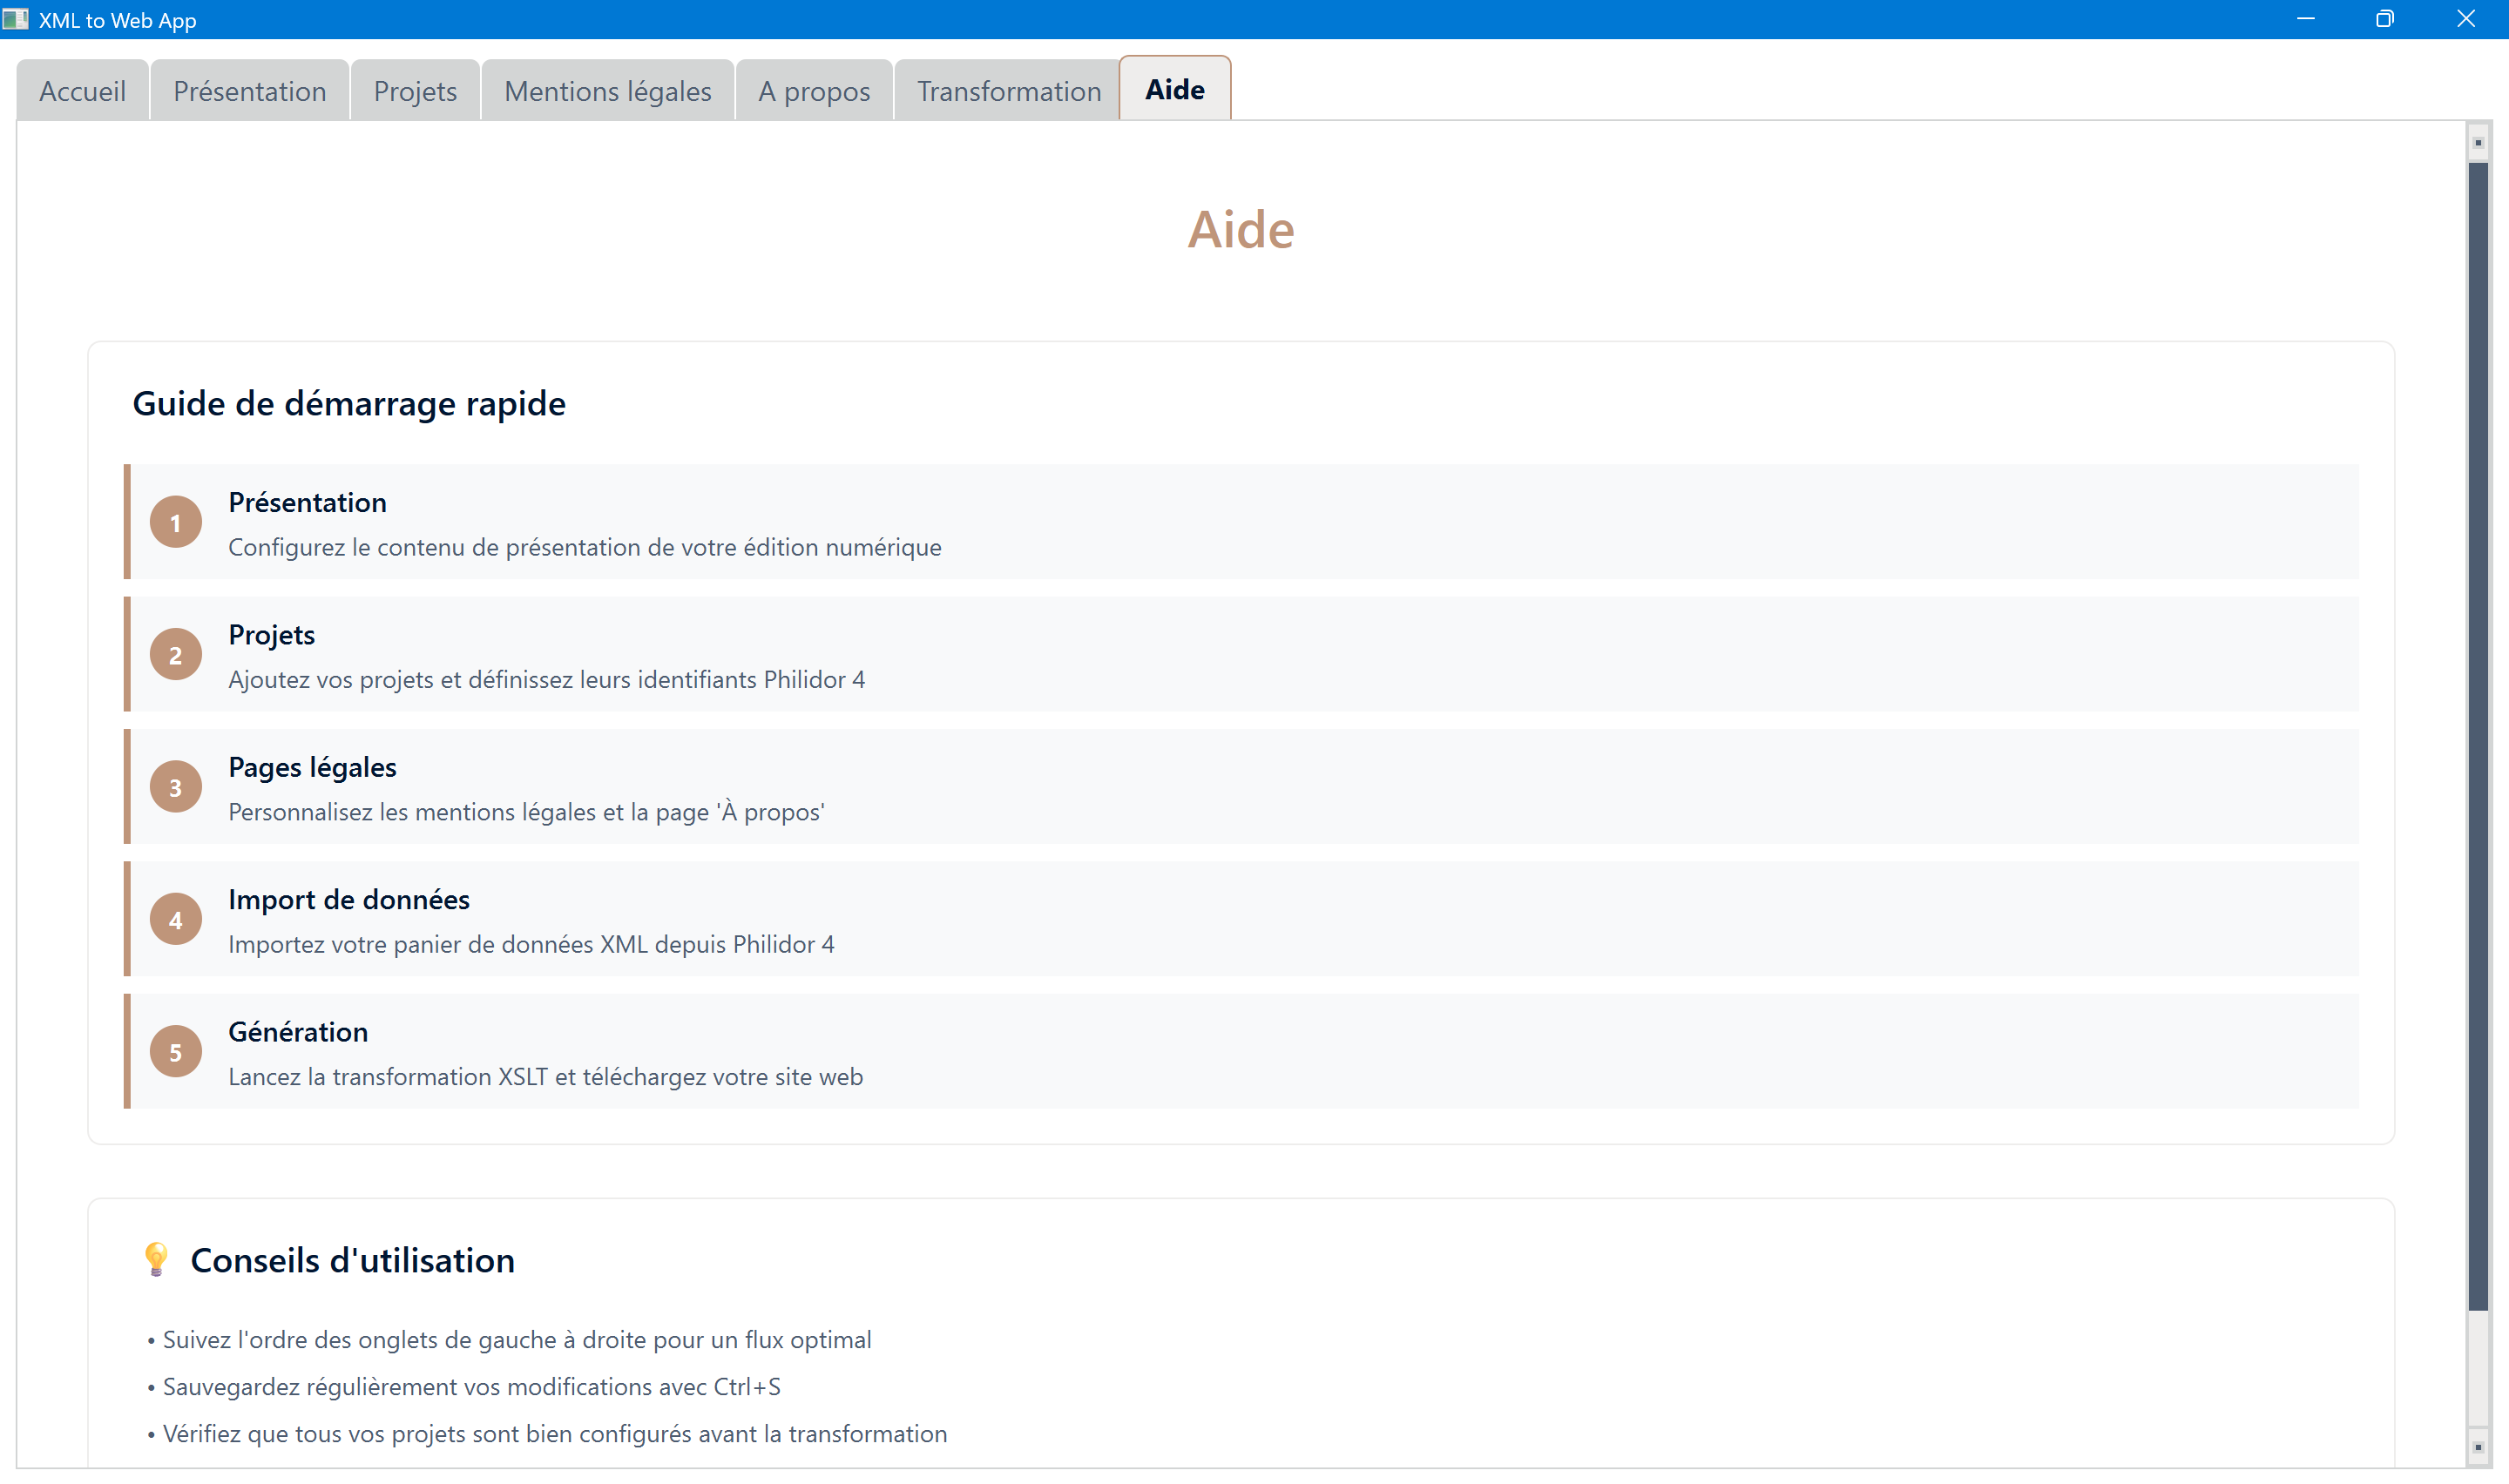
\includegraphics[width=\textwidth]{images/appli-onglet-aide.png}
\end{figure}

\section{Construction du site web avec \gls{xslt}}

La génération automatique d'un site web éditorialisé à partir des données de \textit{Philidor~4} représente un défi technique et éditorial complexe. Cette transformation des données musicologiques brutes en interface web navigable s'articule autour de trois enjeux fondamentaux : la création d'une identité visuelle cohérente avec l'écosystème numérique du \gls{cmbv}, la structuration intelligible des contenus scientifiques, et la gestion des limites inhérentes aux données sources. L'analyse de cette mise en œuvre révèle comment les choix techniques et graphiques façonnent directement l'appropriation des contenus patrimoniaux par les utilisateurs, tout en mettant en évidence les défis persistants de la valorisation numérique des catalogues musicologiques.

\subsection{Navigation générale et charte graphique}

L'intégration visuelle de l'édition web de \textit{Philidor~4} dans l'écosystème numérique du \gls{cmbv} constitue un enjeu majeur d'appropriation et de reconnaissance institutionnelle. Cette cohérence graphique, loin d'être purement cosmétique, participe à la construction d'une identité numérique unifiée qui facilite la navigation des utilisateurs entre les différentes ressources du \glslink{cmbv}{Centre}.

\subsubsection{Éléments d'identité visuelle partagée}

L'architecture générale du site reflète directement la hiérarchie des données musicologiques tout en respectant les codes visuels établis par le \gls{cmbv}. La page d'accueil (cf. figure \ref{accueil-edition}) présente une liste organisée des projets disponibles, accompagnée d'informations quantitatives sur les contenus. Cette approche statistique, générée automatiquement par le template \codeinline{xml}{create-index}, donne immédiatement aux utilisateurs une vision synthétique des corpus disponibles.

\begin{figure}[h]
	\caption{Accueil de l'édition web} \label{accueil-edition}
	\centering
	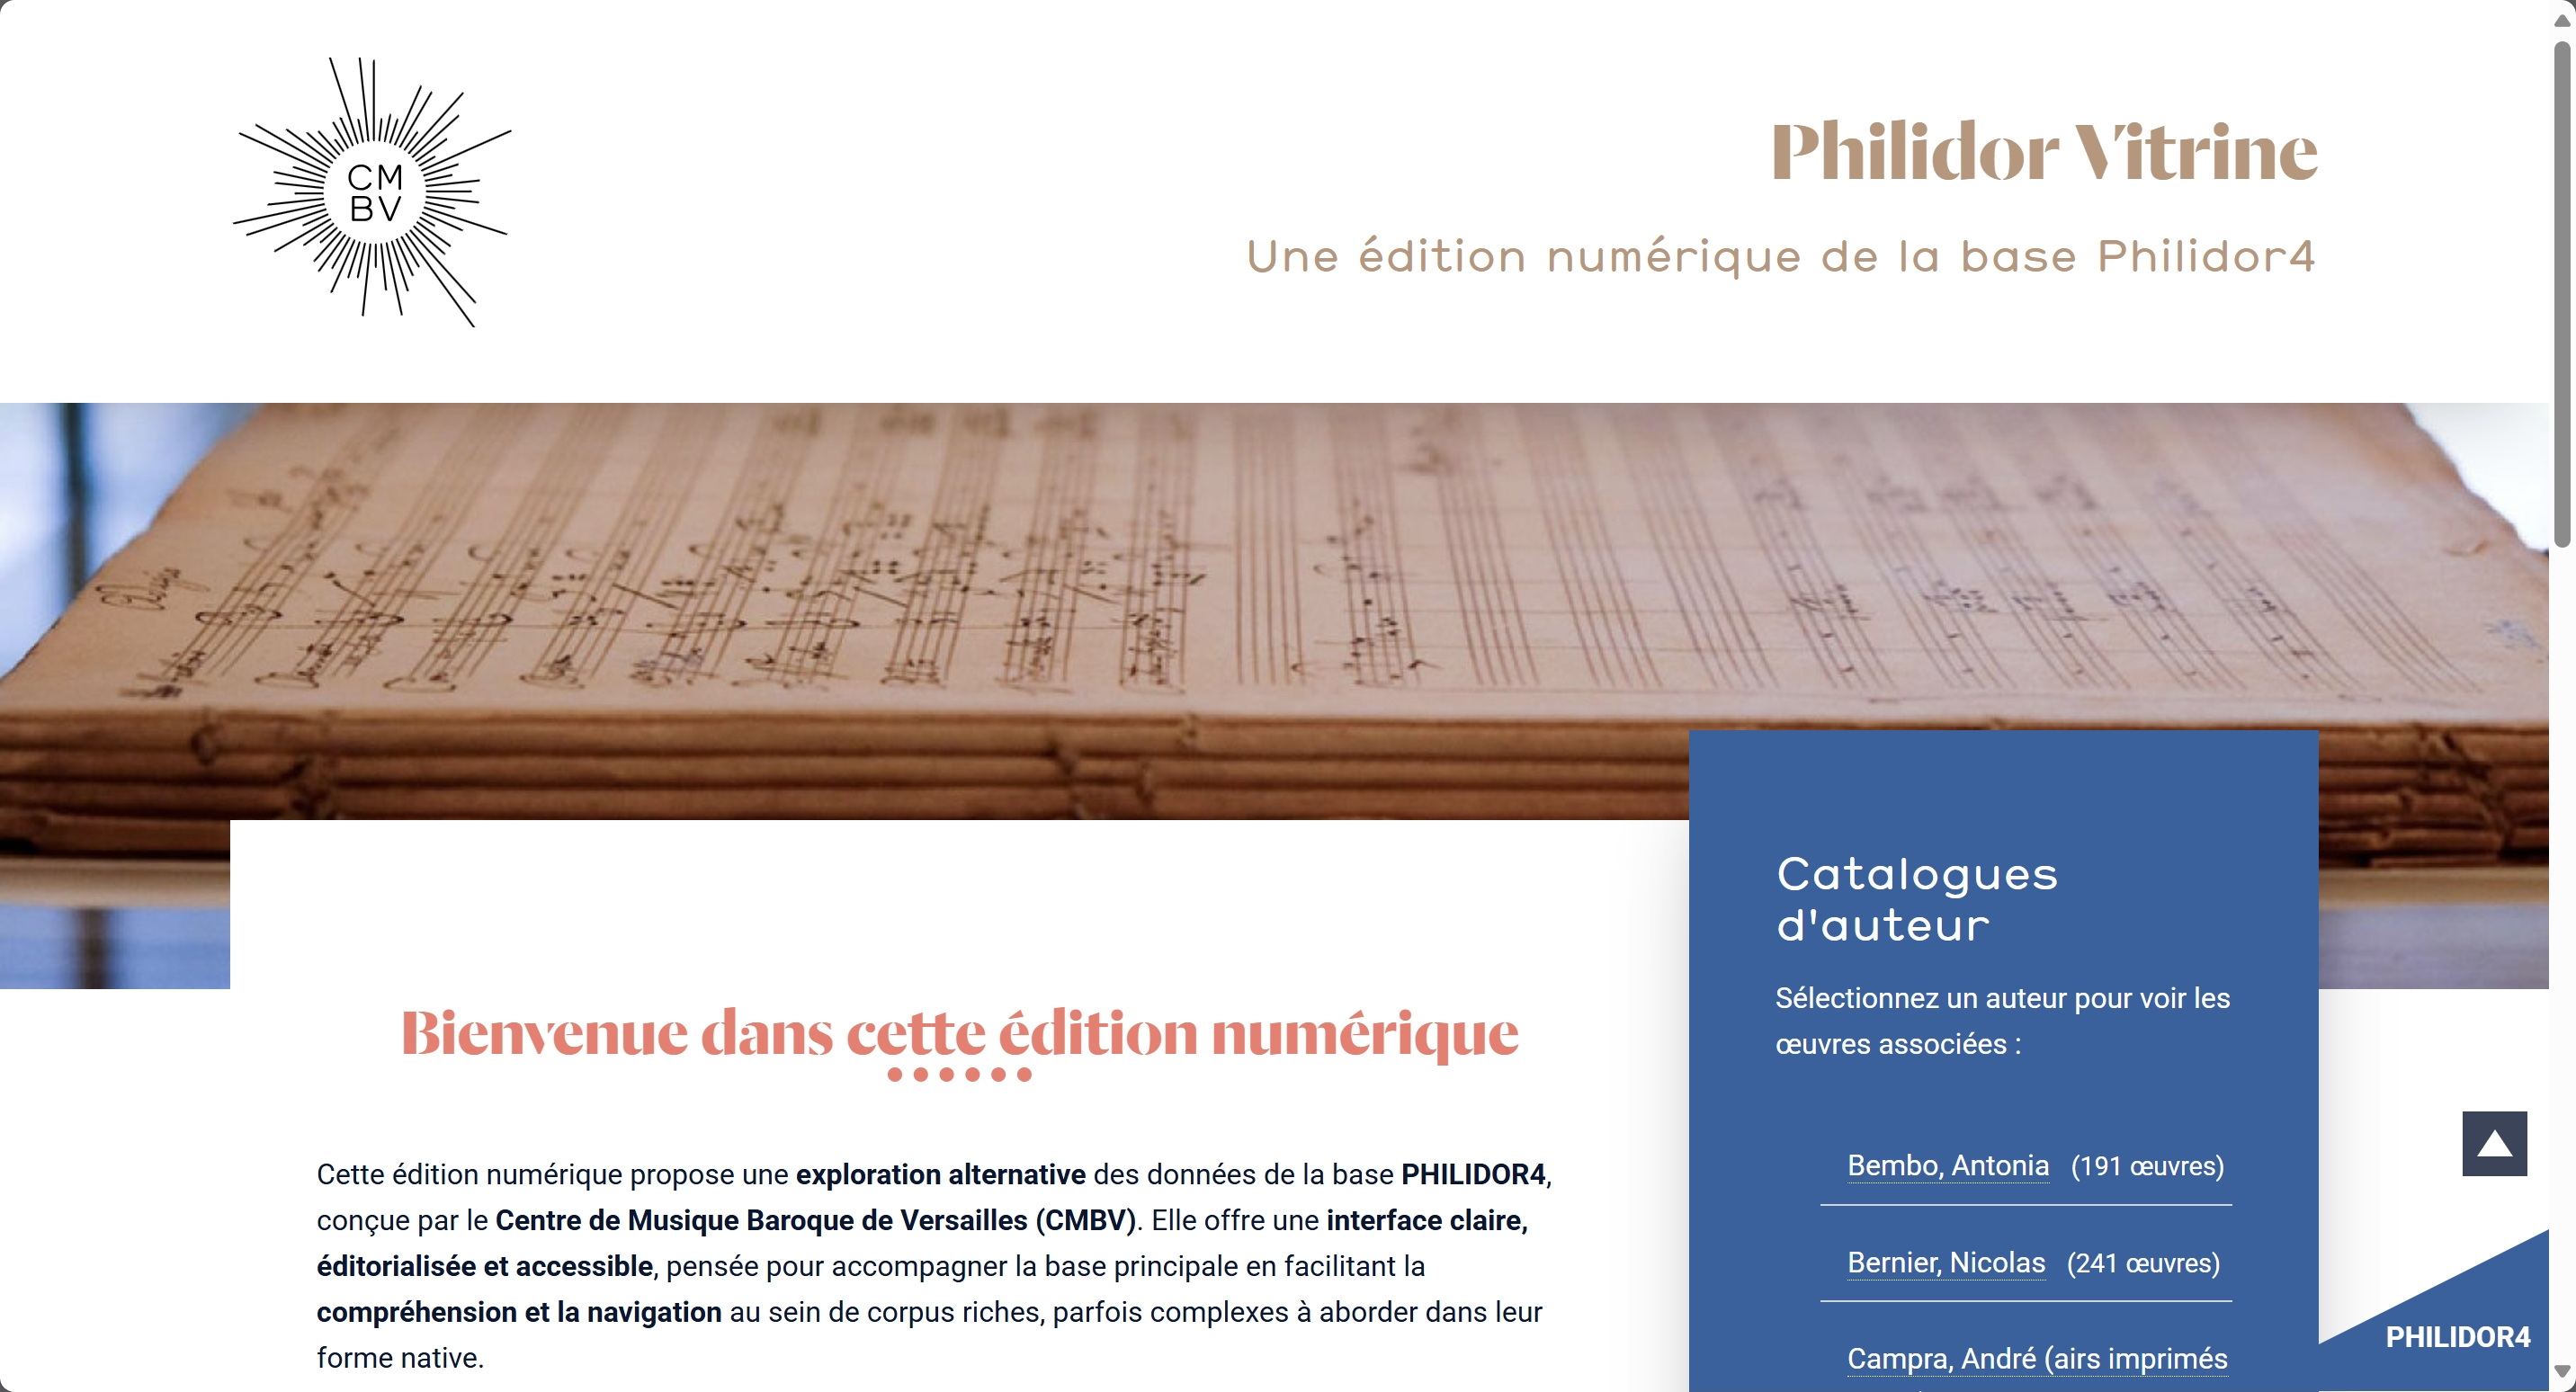
\includegraphics[width=\textwidth]{images/accueil-edition-philidor.png}
\end{figure}

Le header reprend fidèlement l'identité du site officiel du \gls{cmbv} : fond blanc, ombre portée subtile, et intégration du logo soleil animé, reprogrammé intégralement en JavaScript. Ce dernier élément, particulièrement significatif, reproduit exactement le rayonnement animé présent sur tous les sites de l'institution. Plus qu'un simple ornement, il constitue un lien fonctionnel vers la page \textquote{ressources numériques} du \gls{cmbv}, inscrivant ainsi l'édition dans l'écosystème général des outils du \glslink{cmbv}{Centre}.

La cohérence s'étend aux détails interactifs : le footer emprunte sa mise en forme au site officiel, incluant les effets de survol (\textit{hover}) des liens. Les couleurs utilisées respectent scrupuleusement la charte graphique institutionnelle, définies par des variables CSS globales qui reprennent les teintes officielles (cf. figure \ref{couleurs-cmbv}) :

\begin{codeblock}{css}
:root {
    /* Couleurs principales */
    --color-rouge-clair: #f5a8c8;
    --color-rouge: #fd766c;
    --color-rouge-fonce: #b9544e;
    --color-bleu-clair: #5192bd;
    --color-bleu: #0763a1;
    --color-bleu-fonce: #054570;
    --color-nuit-clair: #4d5c70;
    --color-nuit: #001632;
    --color-or: #bf957a;
    --color-or-fonce: #a06d4d;
    --color-gris: #eeedec;
    --color-gris-fonce: #d3d5d5;
    --color-noir: #001632;
    --color-blanc: #fff;
}
\end{codeblock}

\begin{figure}[h]
	\caption{Les couleurs de la chartes graphiques du \gls{cmbv} dans l'ordre listé par les variables ci-dessus} \label{couleurs-cmbv}
	\centering
	
\includegraphics[width=\textwidth]{images/couleurs-cmbv.jpeg}
\end{figure}

\subsubsection{Emprunts et adaptations depuis l'écosystème \gls{cmbv}}

Cette cohérence visuelle procède d'emprunts ciblés aux différents sites du \gls{cmbv}, chaque élément étant adapté au contexte spécifique de l'édition musicologique. Les titres rouges et les liens bleus soulignés en pointillés s'inspirent directement du site \textquote{Découvrir le Baroque}\footnote{cf. \url{https://cmbv.fr/fr/decouvrir-le-baroque}}, établissant une filiation claire avec les ressources pédagogiques du \glslink{cmbv}{Centre}. Cette continuité chromatique facilite l'appropriation par les utilisateurs déjà familiers de l'écosystème \gls{cmbv}.

Les accordéons, élément central de l'organisation des contenus, reproduisent exactement ceux utilisés sur le site principal du \gls{cmbv}. Ils sont notamment visibles sur la page de la bibliothèque\footcite{CentreMusiqueBaroqueb}. Cette uniformisation des interactions garantit une expérience utilisateur fluide et prévisible. Le système d'accordéon, géré par JavaScript, permet de présenter de grandes quantités d'informations structurées sans surcharge visuelle.

Le petit rayon bleu en bas à droite constitue peut-être l'exemple le plus raffiné de cette intégration. Reprenant exactement le graphisme et les animations du rayon web-radio du site principal, il grandit et change de couleur selon les mêmes modalités, tout en redirigeant vers la base de données \textit{Philidor~4} originale. Cette continuité gestuelle renforce l'impression d'un écosystème numérique unifié.

\subsubsection{Architecture de navigation et expérience utilisateur}

La structure de navigation s'organise selon une hiérarchie à trois niveaux qui respecte les logiques de consultation musicologique : accueil général, catalogues de projets, et notices individuelles. Cette organisation arborescente correspond aux habitudes d'exploration des chercheurs, qui commencent généralement par identifier un compositeur avant d'explorer ses œuvres.

\begin{figure}[h]
	\caption{Page du projet sur les sources et oeuvres de la compositrice \textquote{Antonia Bembo}} \label{page-projet-edition}
	\centering
	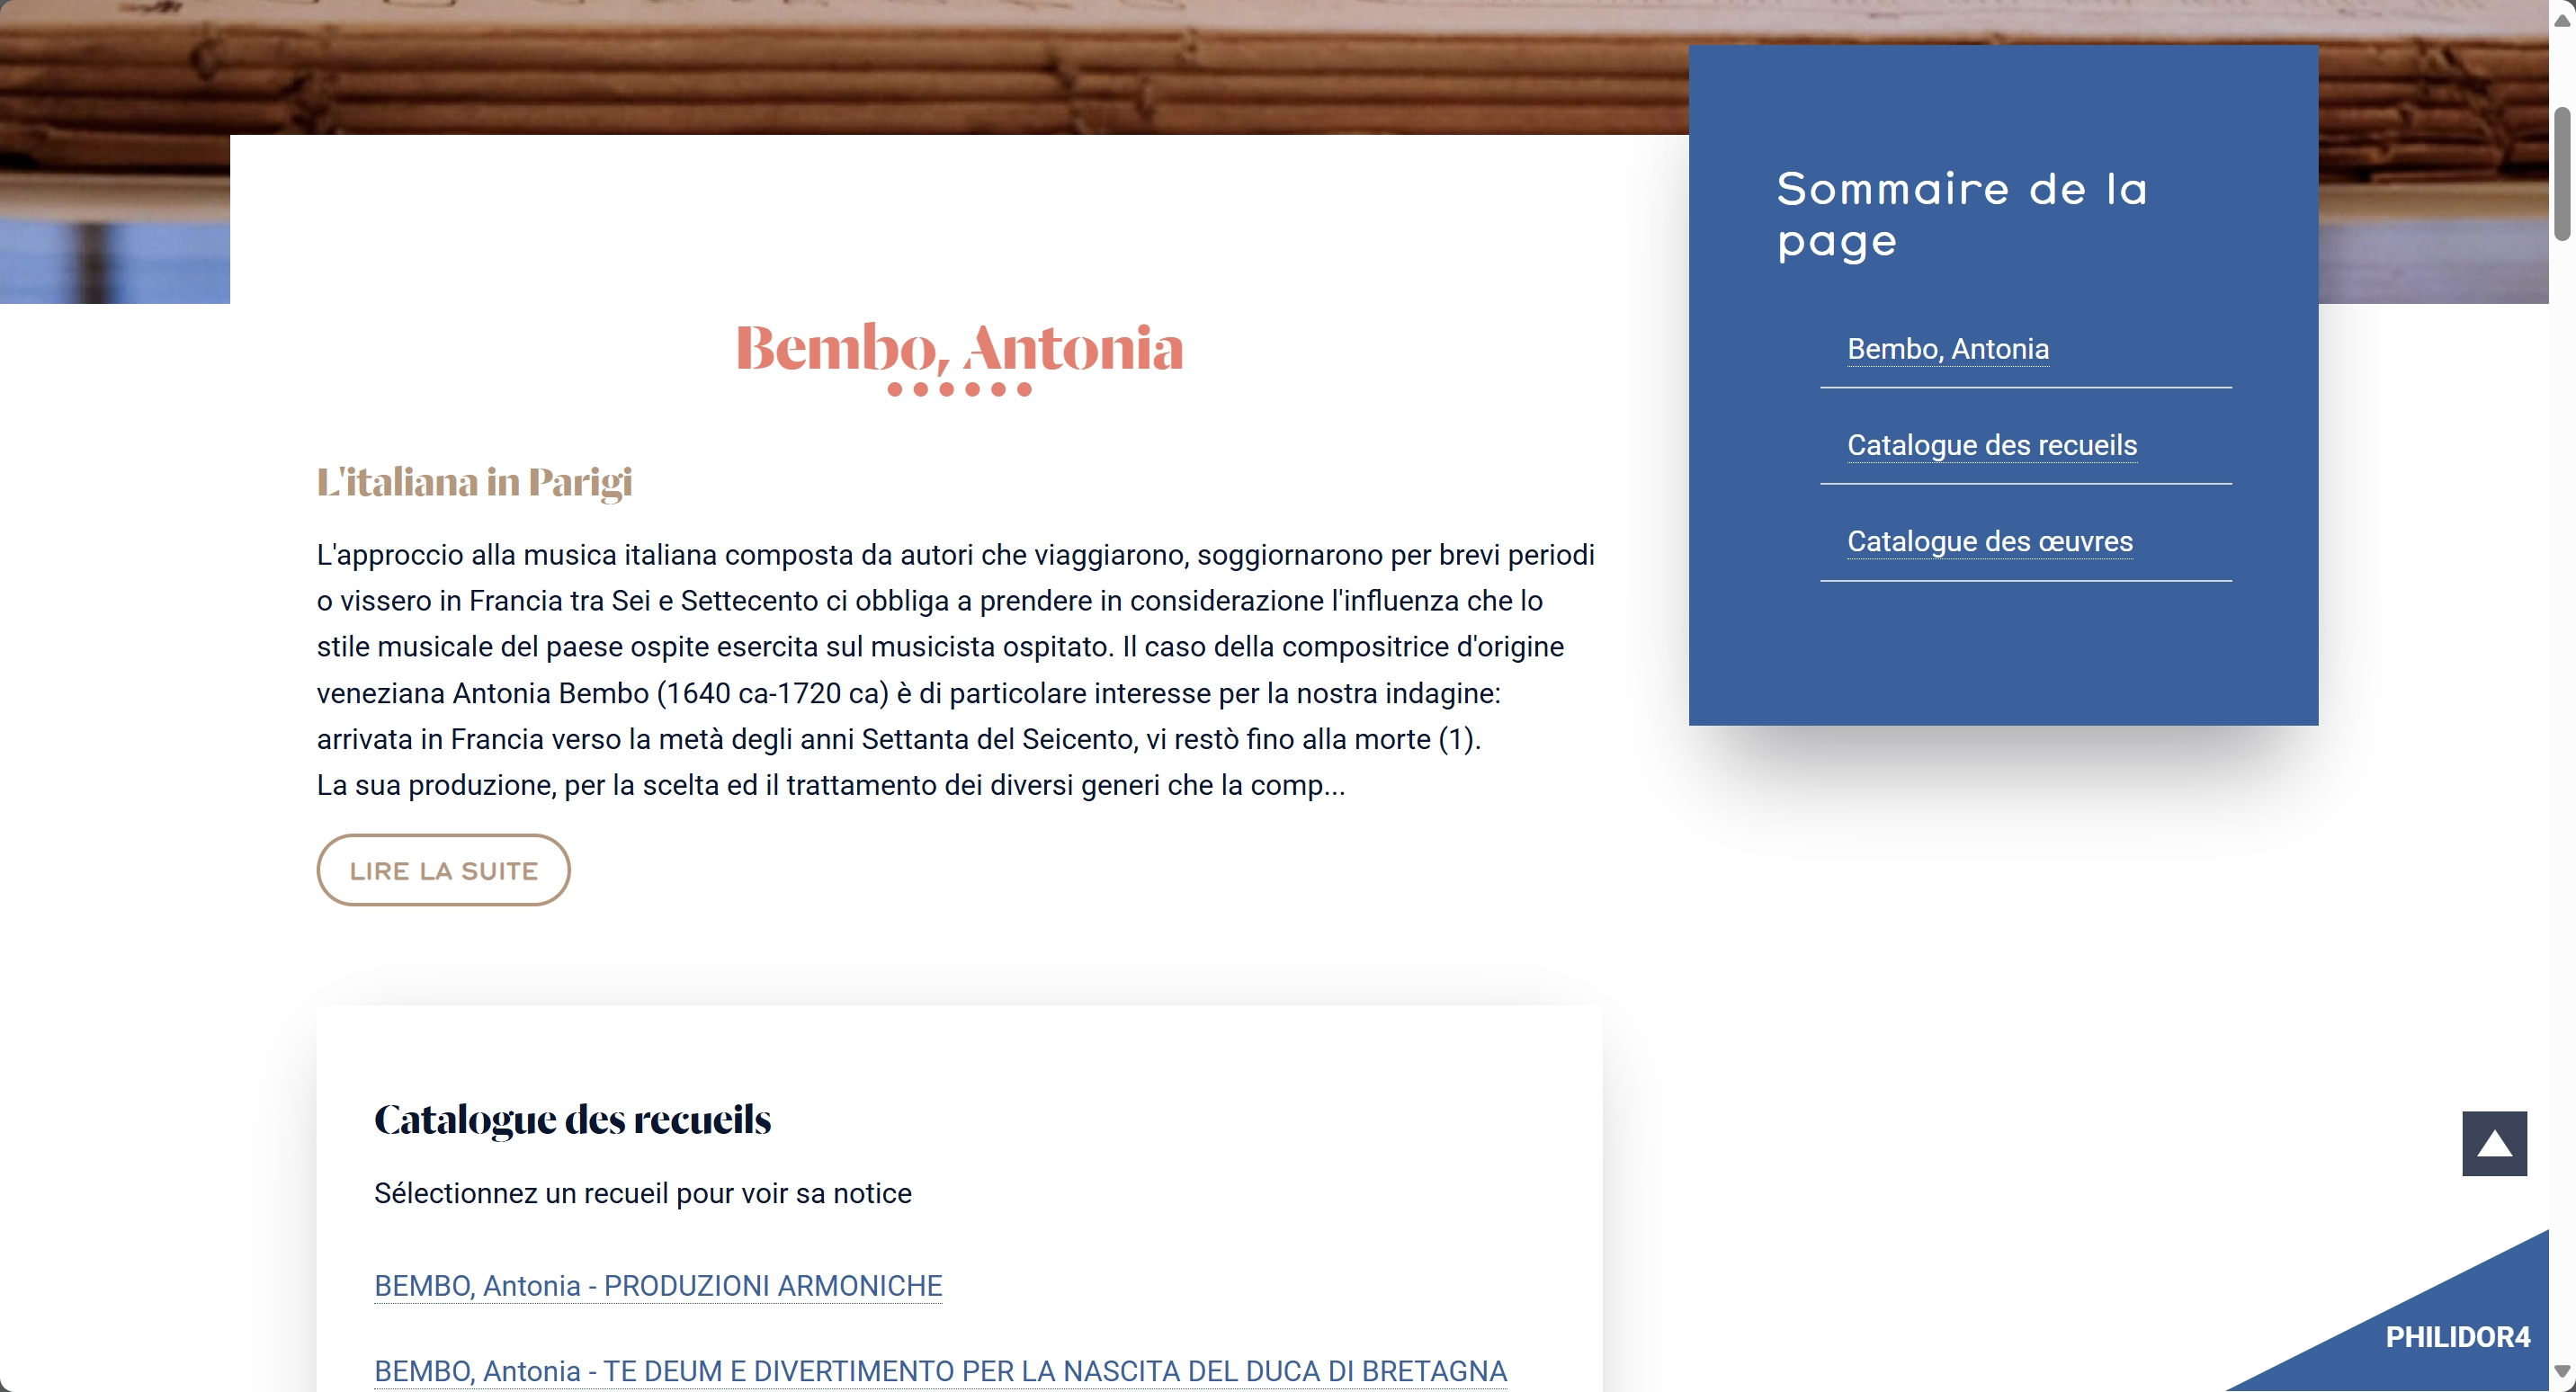
\includegraphics[width=\textwidth]{images/page-bembo-edition-philidor.png}
\end{figure}

Les pages de projet (cf. figure \ref{page-projet-edition}) intègrent un système de sommaire automatique avec ancrage, facilitant la navigation dans des catalogues potentiellement longs. Les liens vers les sections (\codeinline{text}{#project-title}, \codeinline{text}{#recueil-section}, \codeinline{text}{#oeuvre-section}) permettent un accès direct aux différents types de contenus. Cette fonctionnalité, générée automatiquement par les templates \gls{xslt}, s'adapte dynamiquement au contenu de chaque projet. De plus, la description du projet s'affiche tronquée en haut de la page, sous le titre, avec un bouton ramenant en bas de la page, là où se trouve la description complète. Ce mode d'affichage permet d'avoir accès rapidement aux ressources, si la description du projet ne nous intéresse pas. Cette fonctionnalité s'inspire des catalogues en ligne de magasins, comme la FNAC, qui propose un aperçu de la description des produits en haut des notices avec un bouton \textquote{Lire la suite}.

La gestion des chemins relatifs, orchestrée par le paramètre \codeinline{text}{page-path}, assure la cohérence des liens entre les différents niveaux de l'arborescence. Les templates communs (\codeinline{text}{common-head}, \codeinline{text}{common-header}, \codeinline{text}{common-footer}) centralisent les éléments de navigation, évitant la duplication de code tout en garantissant une expérience homogène.

Cette intégration visuelle et fonctionnelle dans l'écosystème \gls{cmbv} prépare le terrain pour la présentation des contenus musicologiques eux-mêmes, dont la structuration nécessite des approches spécialisées adaptées aux différents types d'entités cataloguées.

\subsection{Construction des notices individuelles}

La transformation des données brutes de \textit{Philidor~4} en notices web lisibles représente le cœur technique et éditorial du projet. Cette opération dépasse la simple conversion de format : elle implique des choix de structuration, de présentation et d'organisation qui conditionnent directement l'appropriation des contenus par les utilisateurs\footcite{chartronEditionPublicationContenus2016}. L'analyse de cette construction révèle les stratégies adoptées pour rendre accessible la complexité des données musicologiques tout en préservant leur richesse scientifique.

\subsubsection{Logique de différenciation par types d'entités}

La feuille de transformation distingue trois types de notices correspondant aux entités principales de \textit{Philidor~4} : œuvres, sources et fragments. Cette typologie détermine des modes de présentation spécialisés.

\begin{figure}[p]
	\caption{Une notice d'œuvre} \label{notice-edition}
	\centering
	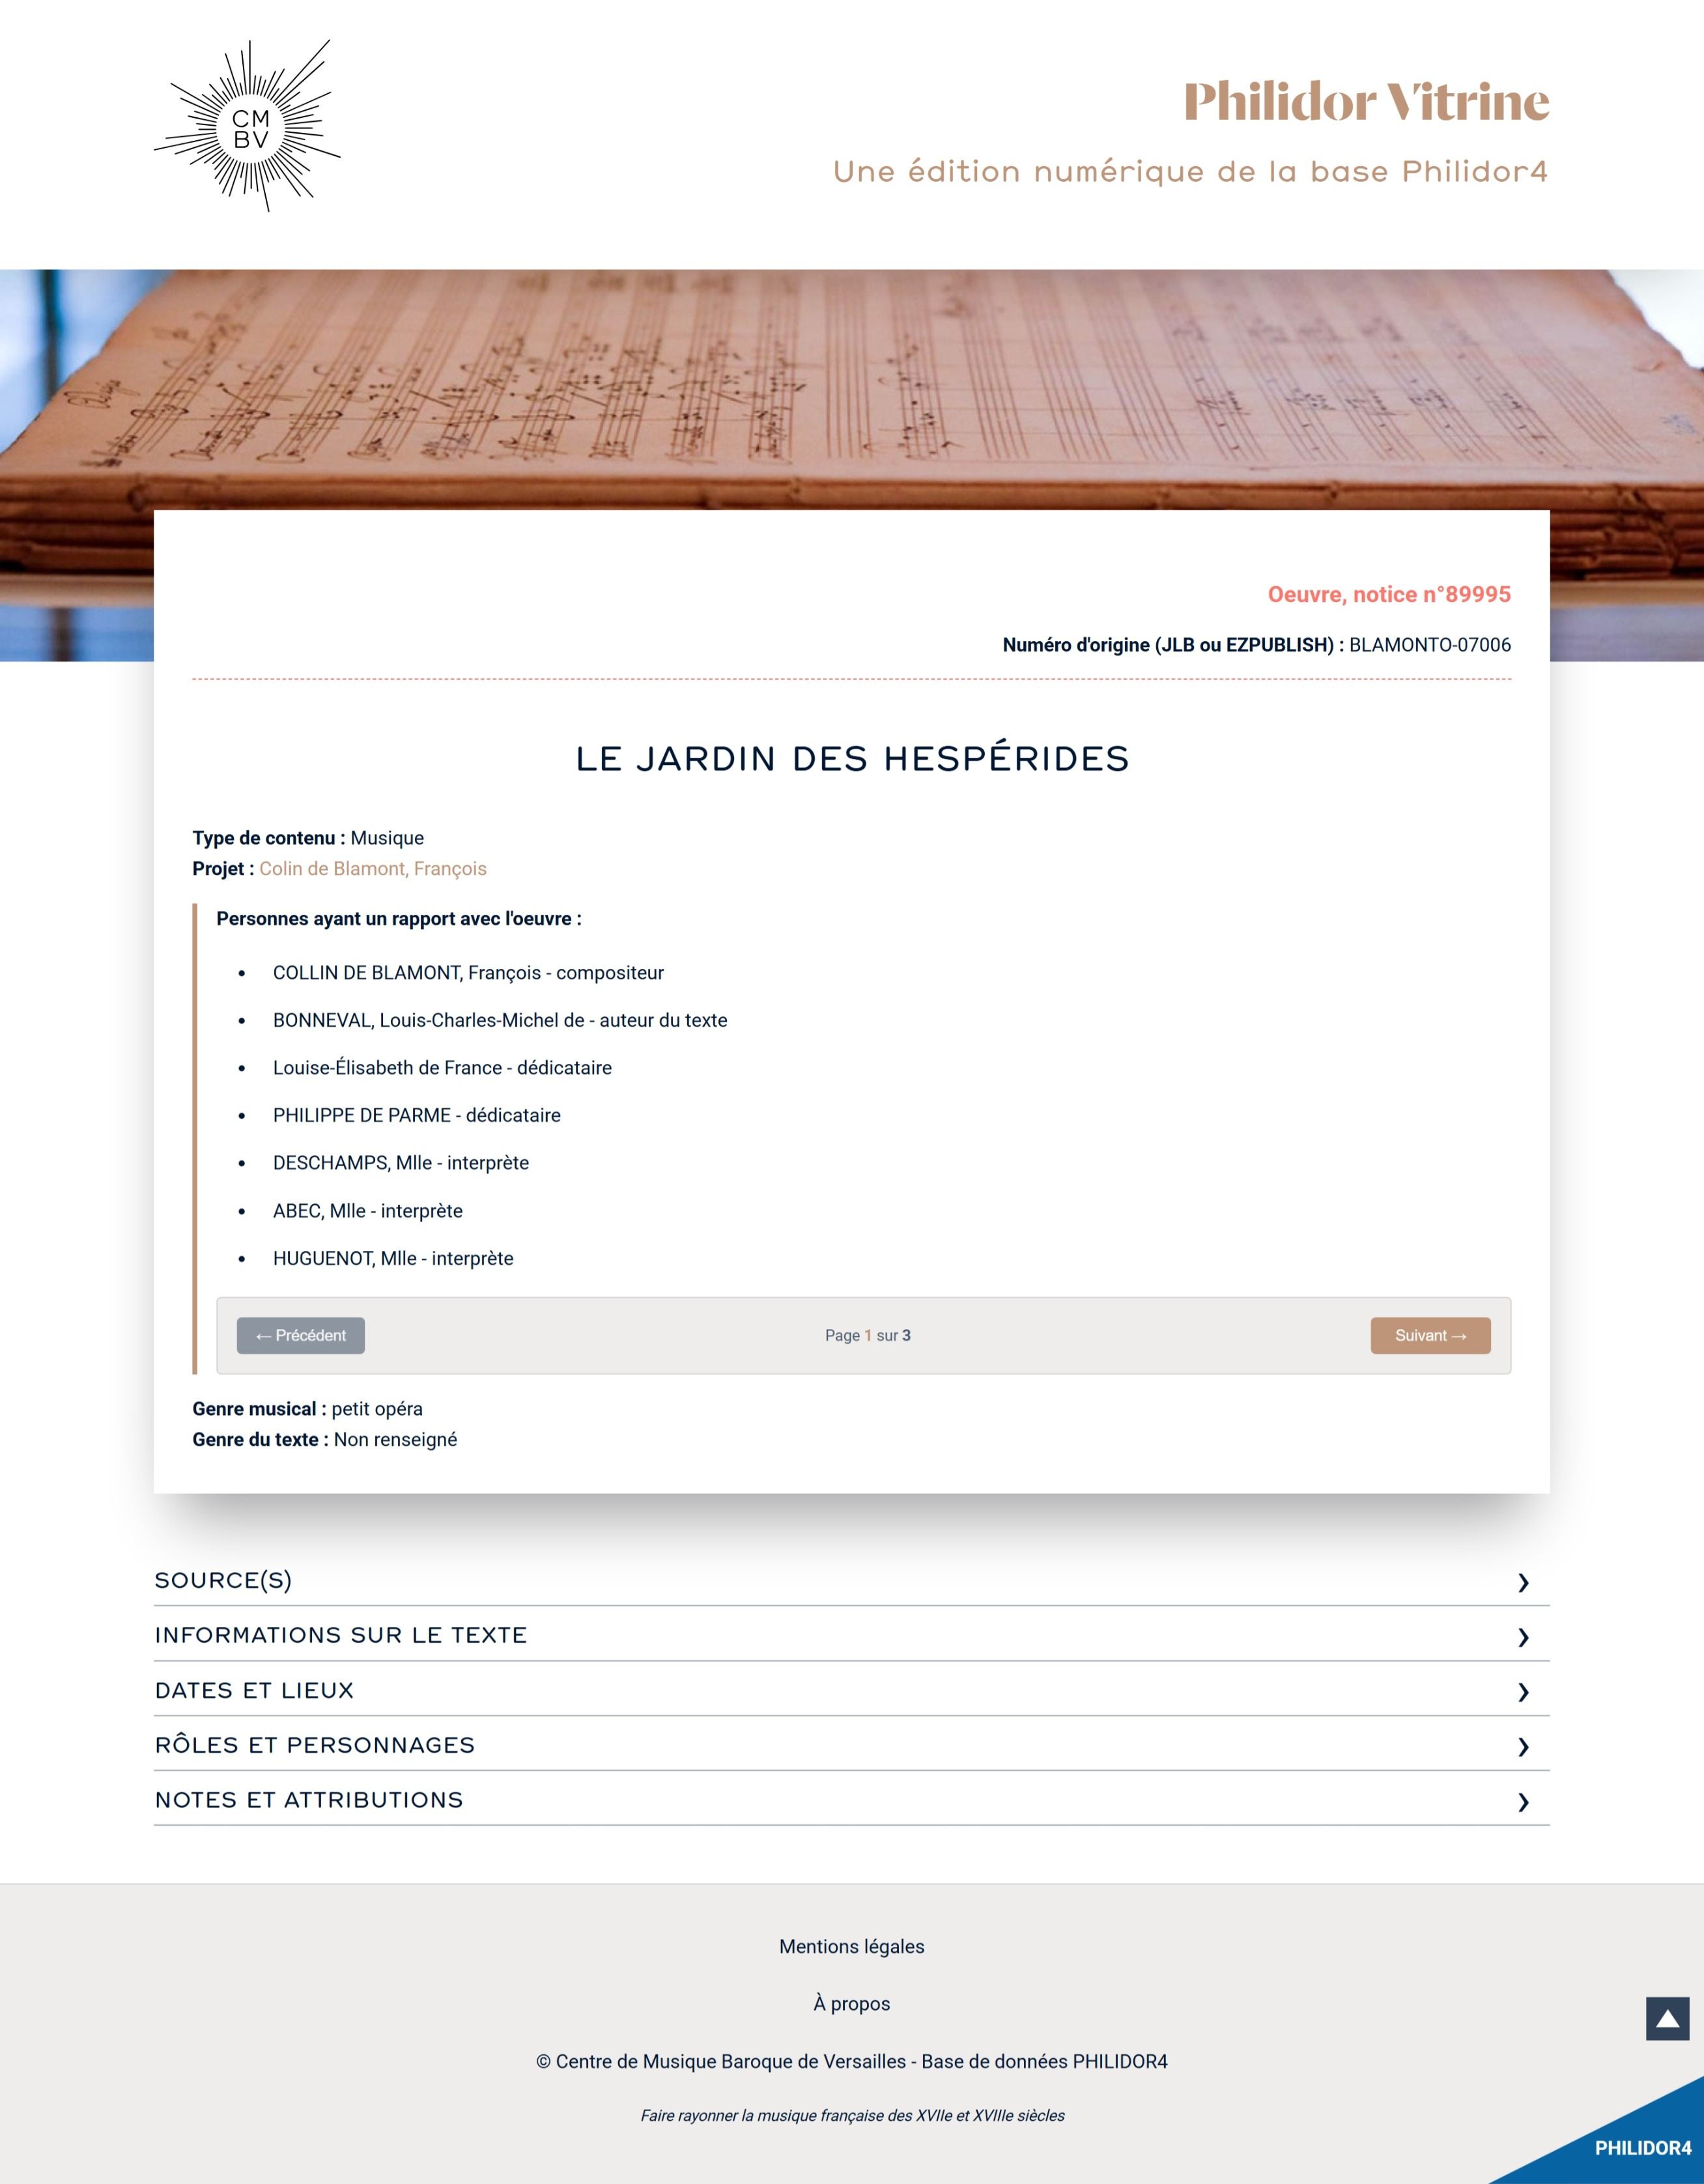
\includegraphics[width=\textwidth]{images/exemple-notice1-edition-philidor.jpeg}
\end{figure}

Les notices d'œuvres (cf. figure \ref{notice-edition}) privilégient la présentation du titre principal et de la structure musicale. Le template \codeinline{text}{create-work-page} gère les cas de données incomplètes par une cascade de récupération pour le titre qui est parfois absent : titre principal (\codeinline{text}{oeuvre}), puis titres alternatifs, enfin message d'erreur explicite en cas d'absence totale. Cette approche préventive évite les pages vides tout en signalant aux utilisateurs les lacunes des données sources.

Les notices de sources adoptent une hiérarchie différente afin de récupérer un titre, privilégiant les champs bibliographiques spécialisés (\codeinline{text}{titre_cle_sre}, \codeinline{text}{notice_bibl}) adaptés aux pratiques de catalogage des documents historiques. Cette différenciation respecte les habitudes disciplinaires tout en optimisant la présentation selon le type de contenu.

Cette approche différenciée garantit que chaque type d'entité bénéficie d'une présentation optimisée selon ses spécificités informationnelles.

\subsubsection{Esthétique de la fiche papier et organisation accordéon}

Le choix esthétique de la fiche d'informations principales constitue l'un des éléments les plus significatifs de l'interface. Cette section, mise en valeur par une ombre portée subtile, évoque les fiches cartonnées qui constituaient autrefois l'outil principal des catalogues de bibliothèque : rangées dans des tiroirs métalliques, ces fiches normalisées permettaient aux chercheurs de consulter rapidement les informations essentielles d'identification de chaque document. L'ombre portée reproduit visuellement cet effet de fiches que l'on pourrait saisir, créant une continuité esthétique entre les pratiques documentaires traditionnelles et l'interface numérique contemporaine.

Cette fiche présente les informations essentielles dans un format condensé (cf. figure \ref{notice-edition}) : titre, personnes impliqués sous la forme d'un carrousel, effectif principal, et données de catalogage. Sa position en tête de notice garantit un accès immédiat aux éléments d'identification, même en cas de contenu très développé. L'ombre portée, subtile mais perceptible, la détache visuellement du reste du contenu tout en créant un effet de profondeur.

L'organisation du contenu complémentaire suit un modèle en accordéon qui permet de présenter de grandes quantités d'informations structurées sans surcharge visuelle (cf. figure \ref{notice-edition}). Les sections se déploient selon une logique musicologique cohérente : incipits, effectif et instrumentation, sources, informations textuelles, références. Cette séquence respecte les habitudes de consultation des chercheurs tout en permettant un accès sélectif aux différents types d'informations.

Le template \codeinline{text}{accordeon} génère automatiquement ces sections, mais ne produit de contenu \gls{html} que si les données correspondantes existent dans le \gls{xml} source. Cette approche évite les sections vides tout en maintenant une structure prévisible. L'interaction JavaScript permet aux utilisateurs de contrôler leur parcours de lecture, dépliant uniquement les sections qui les intéressent.

\subsubsection{Gestion des relations œuvre-fragments}

La reconstitution des liens entre œuvres et fragments représente l'un des défis techniques les plus complexes du projet. Ces relations, essentielles à la compréhension musicologique, nécessitent des stratégies algorithmiques avancées pour être reconstituées à partir des données de \textit{Philidor~4}.

\begin{figure}[h]
	\caption{La notice de l'opéra \textit{Ercole Amante} avec l'affichage de ses fragments en tant que liens hypertextes} \label{notice-ercole-edition}
	\centering
	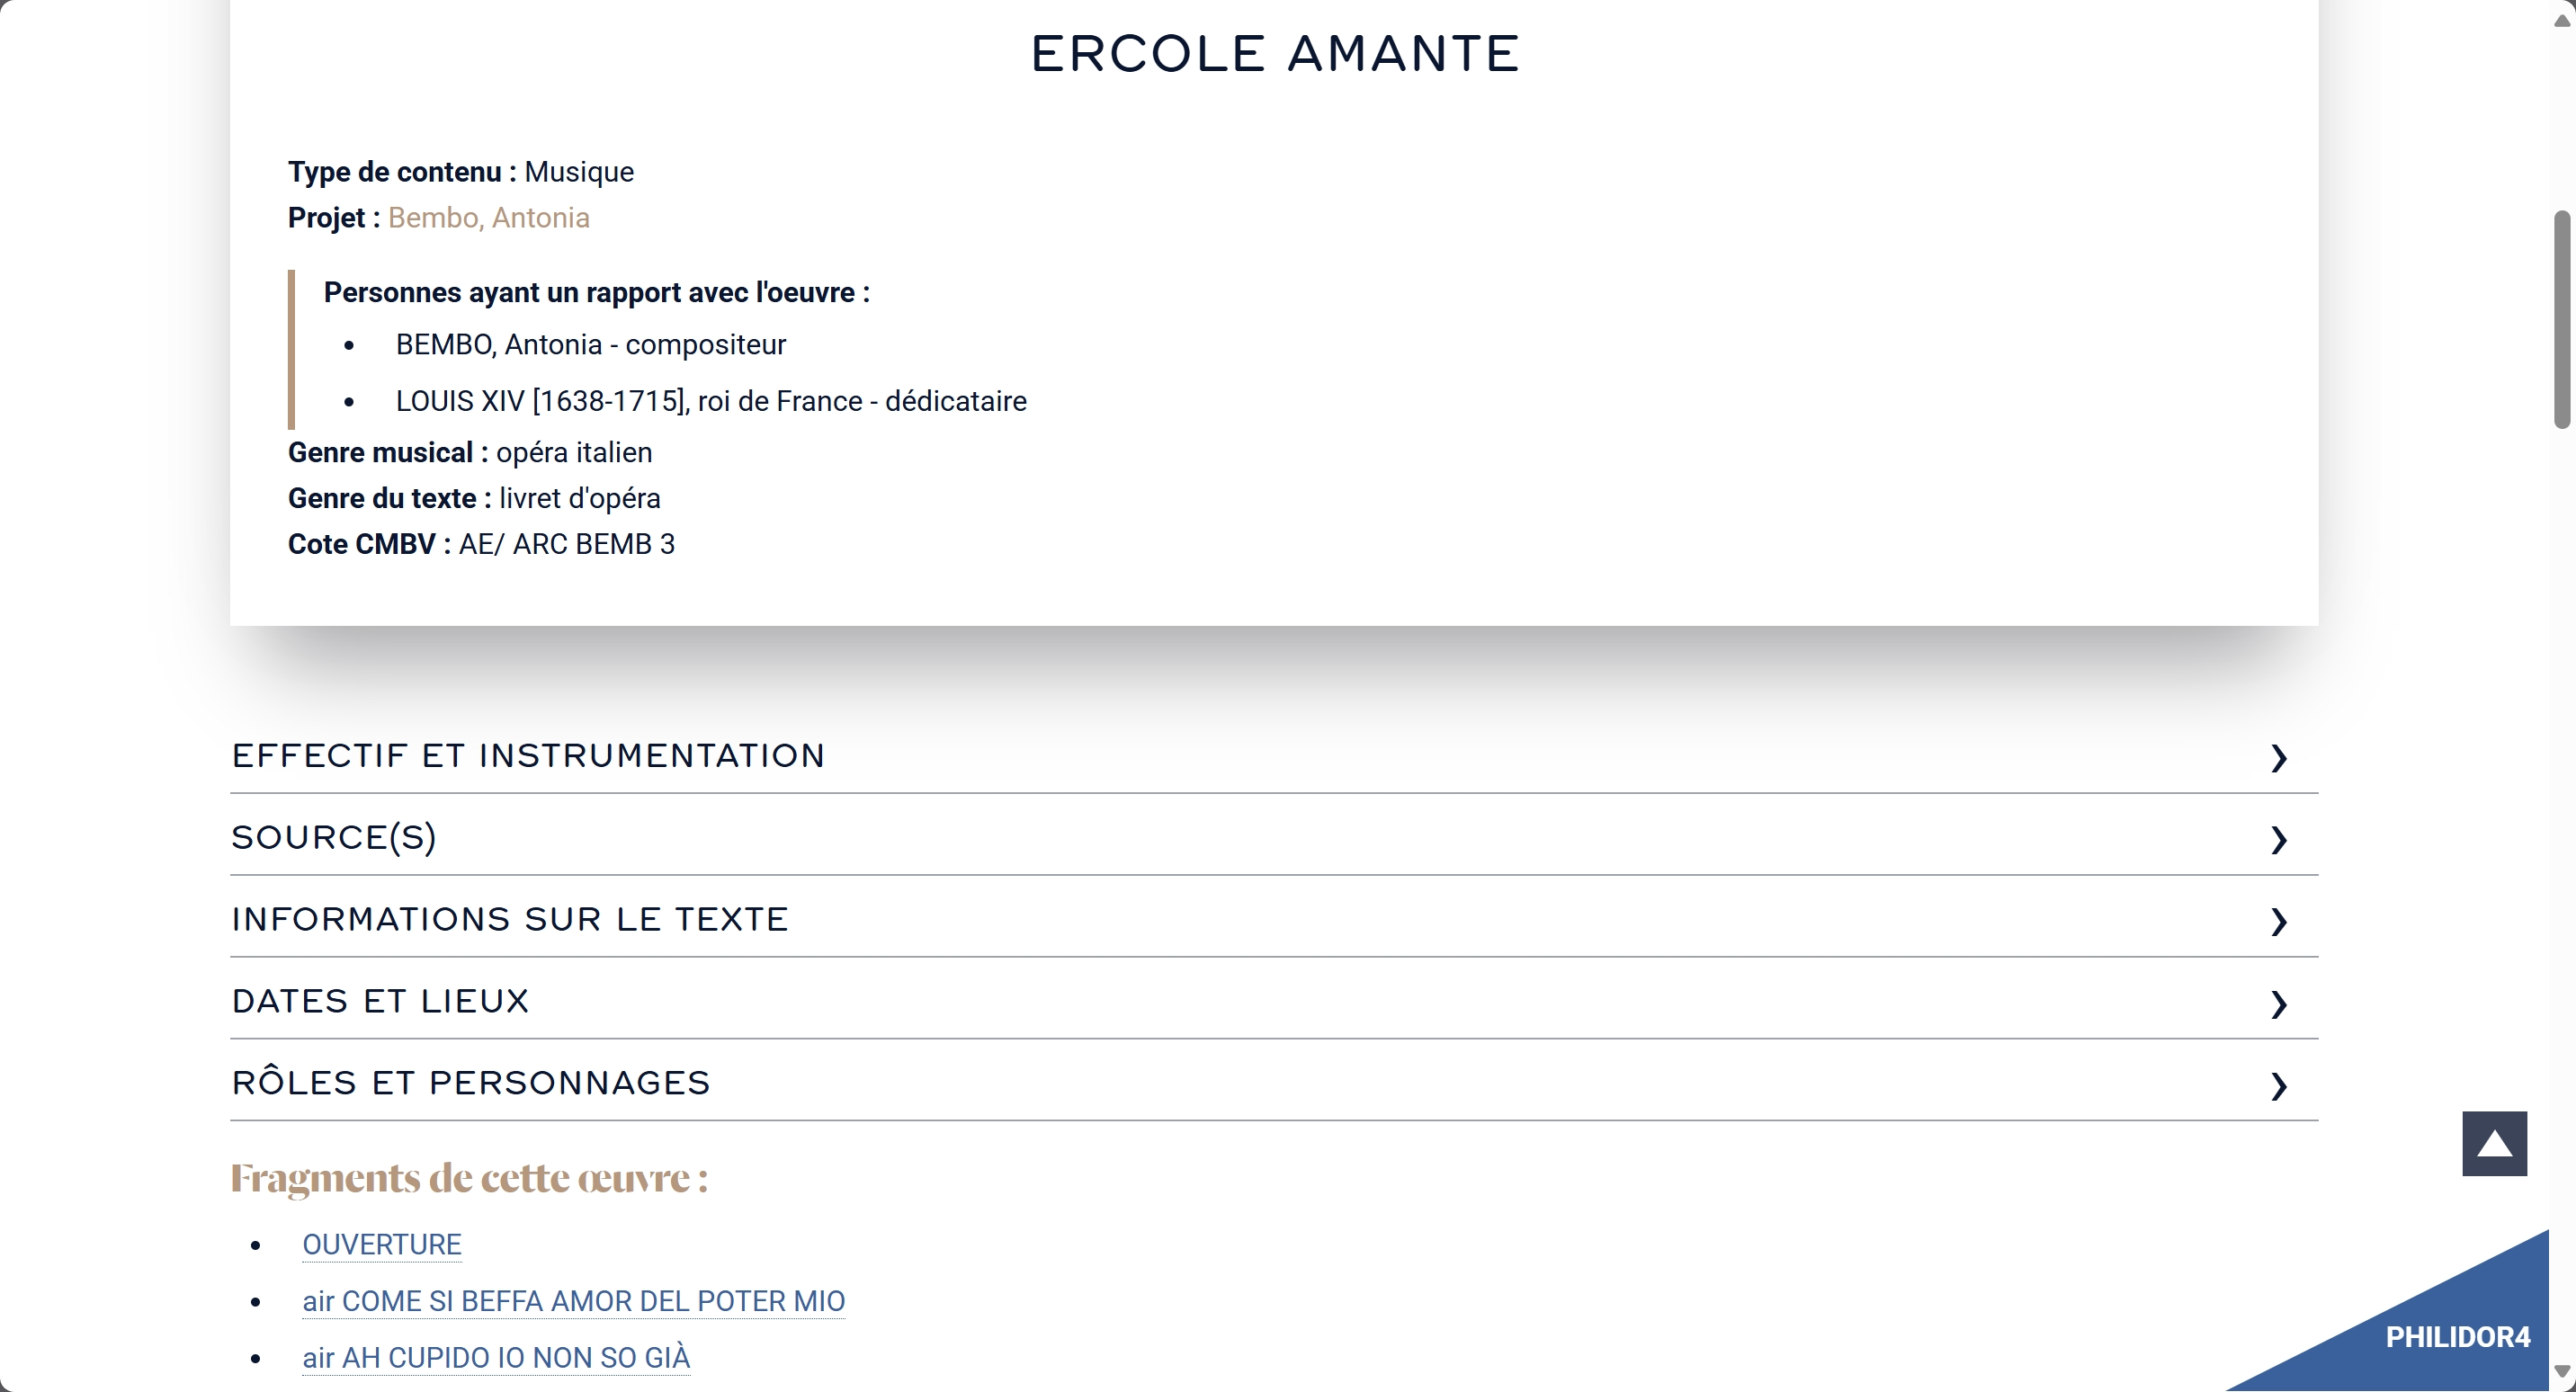
\includegraphics[width=\textwidth]{images/ercole-amante-edition-philidor.png}
\end{figure}

Le template \codeinline{text}{liste-fragments-oeuvre} illustre cette complexité : il décompose la chaîne \codeinline{text}{a_pour_fragments} avec la fonction \codeinline{text}{tokenize()}, puis itère sur chaque identifiant pour retrouver les fragments correspondants dans l'arbre XML. Cette reconstitution, invisible pour l'utilisateur final, permet d'afficher en bas de chaque notice d'œuvre la liste de ses fragments sous forme de liens hypertextuels (cf. figure \ref{notice-ercole-edition}).

\begin{figure}[p]
	\caption{La notice du fragment correspondant à l'ouverture de l'opéra \textit{Ercole Amante}} \label{notice-ercole-frag-edition}
	\centering
	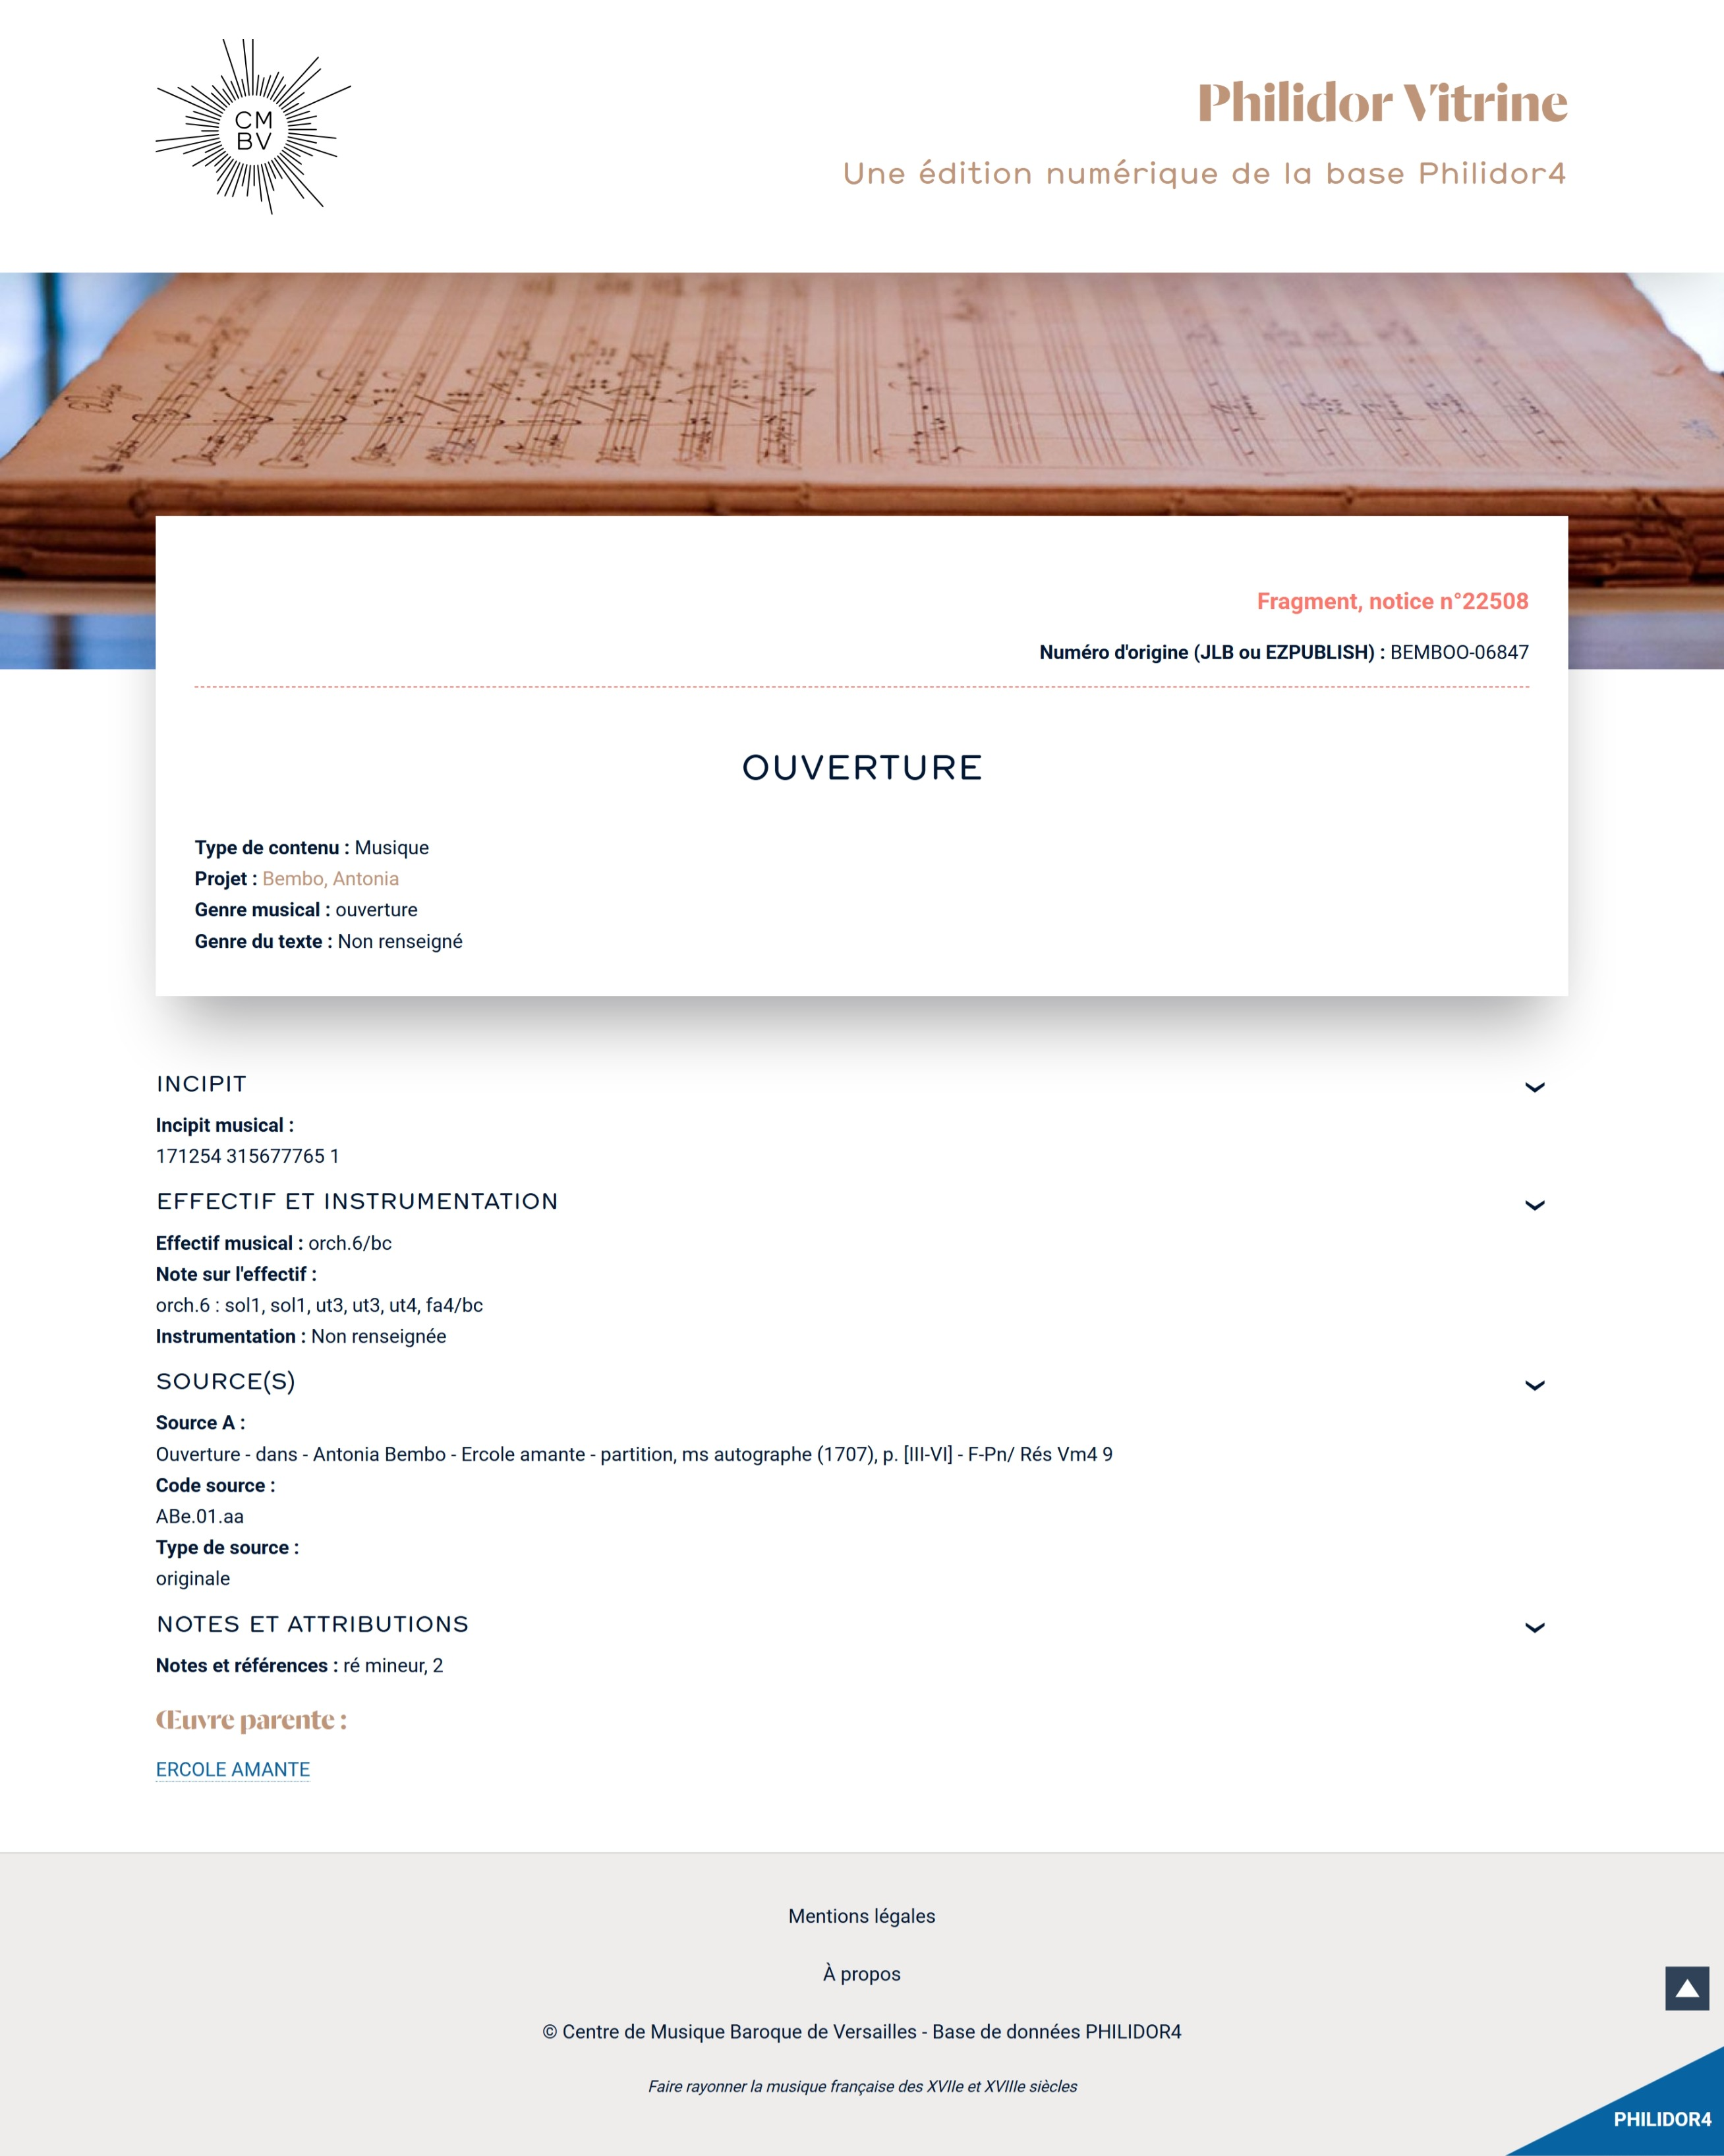
\includegraphics[width=\textwidth]{images/ercole-amante-frag-edition-philidor.jpeg}
\end{figure}

\begin{codeblock}{xml}
<xsl:variable name="fragments-ids" select="tokenize(a_pour_fragments, ' - ')"/>
<xsl:for-each select="$fragments-ids[position() &gt; 1]">
    <xsl:variable name="fragment-number" select="normalize-space(.)"/>
    <!-- recherche du fragment correspondant -->
</xsl:for-each>
\end{codeblock}

Le sens inverse de la relation, géré par le template \codeinline{text}{oeuvre-parente-fragment}, permet aux notices de fragments d'afficher un lien vers leur œuvre parente (cf. figure \ref{notice-ercole-frag-edition}). Cette bidirectionnalité facilite la navigation entre les niveaux hiérarchiques.

La technique de correspondance par suffixe numérique, nécessaire pour faire le lien entre les identifiants textuels et les numéros de notice, révèle la logique de numérotation interne de \textit{Philidor~4}. Cette approche, bien que fonctionnelle, souligne les difficultés inhérentes au traitement de données musicologiques non initialement conçues pour la publication web.

Cette construction sophistiquée des notices individuelles, malgré ses réussites techniques et esthétiques, révèle également les limites du processus de transformation automatique. Ces contraintes, loin d'être purement techniques, soulignent les enjeux plus larges de la valorisation numérique des catalogues musicologiques.

\subsection{Limites observées et avenir du projet}

L'expérience de génération automatique de l'édition web révèle les tensions inhérentes à la transformation de données musicologiques complexes en interface grand public. Ces limites, techniques et épistémologiques, éclairent les défis persistants de la valorisation numérique des patrimoines savants tout en ouvrant des perspectives d'évolution pour le projet.

\subsubsection{Contraintes de normalisation et qualité des données}

La reconstitution des relations entre œuvres et sources s'avère particulièrement problématique en raison de la non-normalisation des données d'origine. Contrairement aux liens œuvre-fragments, qui bénéficient de champs dédiés, les relations avec les sources demeurent largement implicites dans \textit{Philidor~4}. Cette lacune structurelle empêche la génération automatique de liens croisés pourtant essentiels à l'exploitation scientifique des catalogues.

Les titres excessivement longs posent un défi différent mais non moins complexe. Le template \codeinline{text}{format-notice-ligne} tente une normalisation par remplacement des barres obliques et des retours à la ligne par des points médians, reproduisant ainsi les conventions typographiques des ouvrages imprimés historiques. Cette solution, bien qu'imparfaite, améliore sensiblement la lisibilité des références bibliographiques complexes :

\begin{codeblock}{xml}
<xsl:variable name="remplace-slash" select="replace($tronque, ' / ', ' · ')"/>
<xsl:variable name="remplace-retours" select="replace($remplace-slash, '[&#xD;&#xA;]+', ' · ')"/>
\end{codeblock}

Les titres vides ou aberrants constituent une autre limite significative (cf. figure \ref{titre-vide-edition}). Certaines notices, trop pauvres pour générer un titre significatif, affichent des mentions d'erreur explicites. Cette situation révèle les inégalités de documentation des corpus sources et souligne la nécessité d'un travail d'enrichissement préalable à toute valorisation numérique.

\begin{figure}[h]
	\caption{Une notice d'œuvre dont le titre est vide} \label{titre-vide-edition}
	\centering
	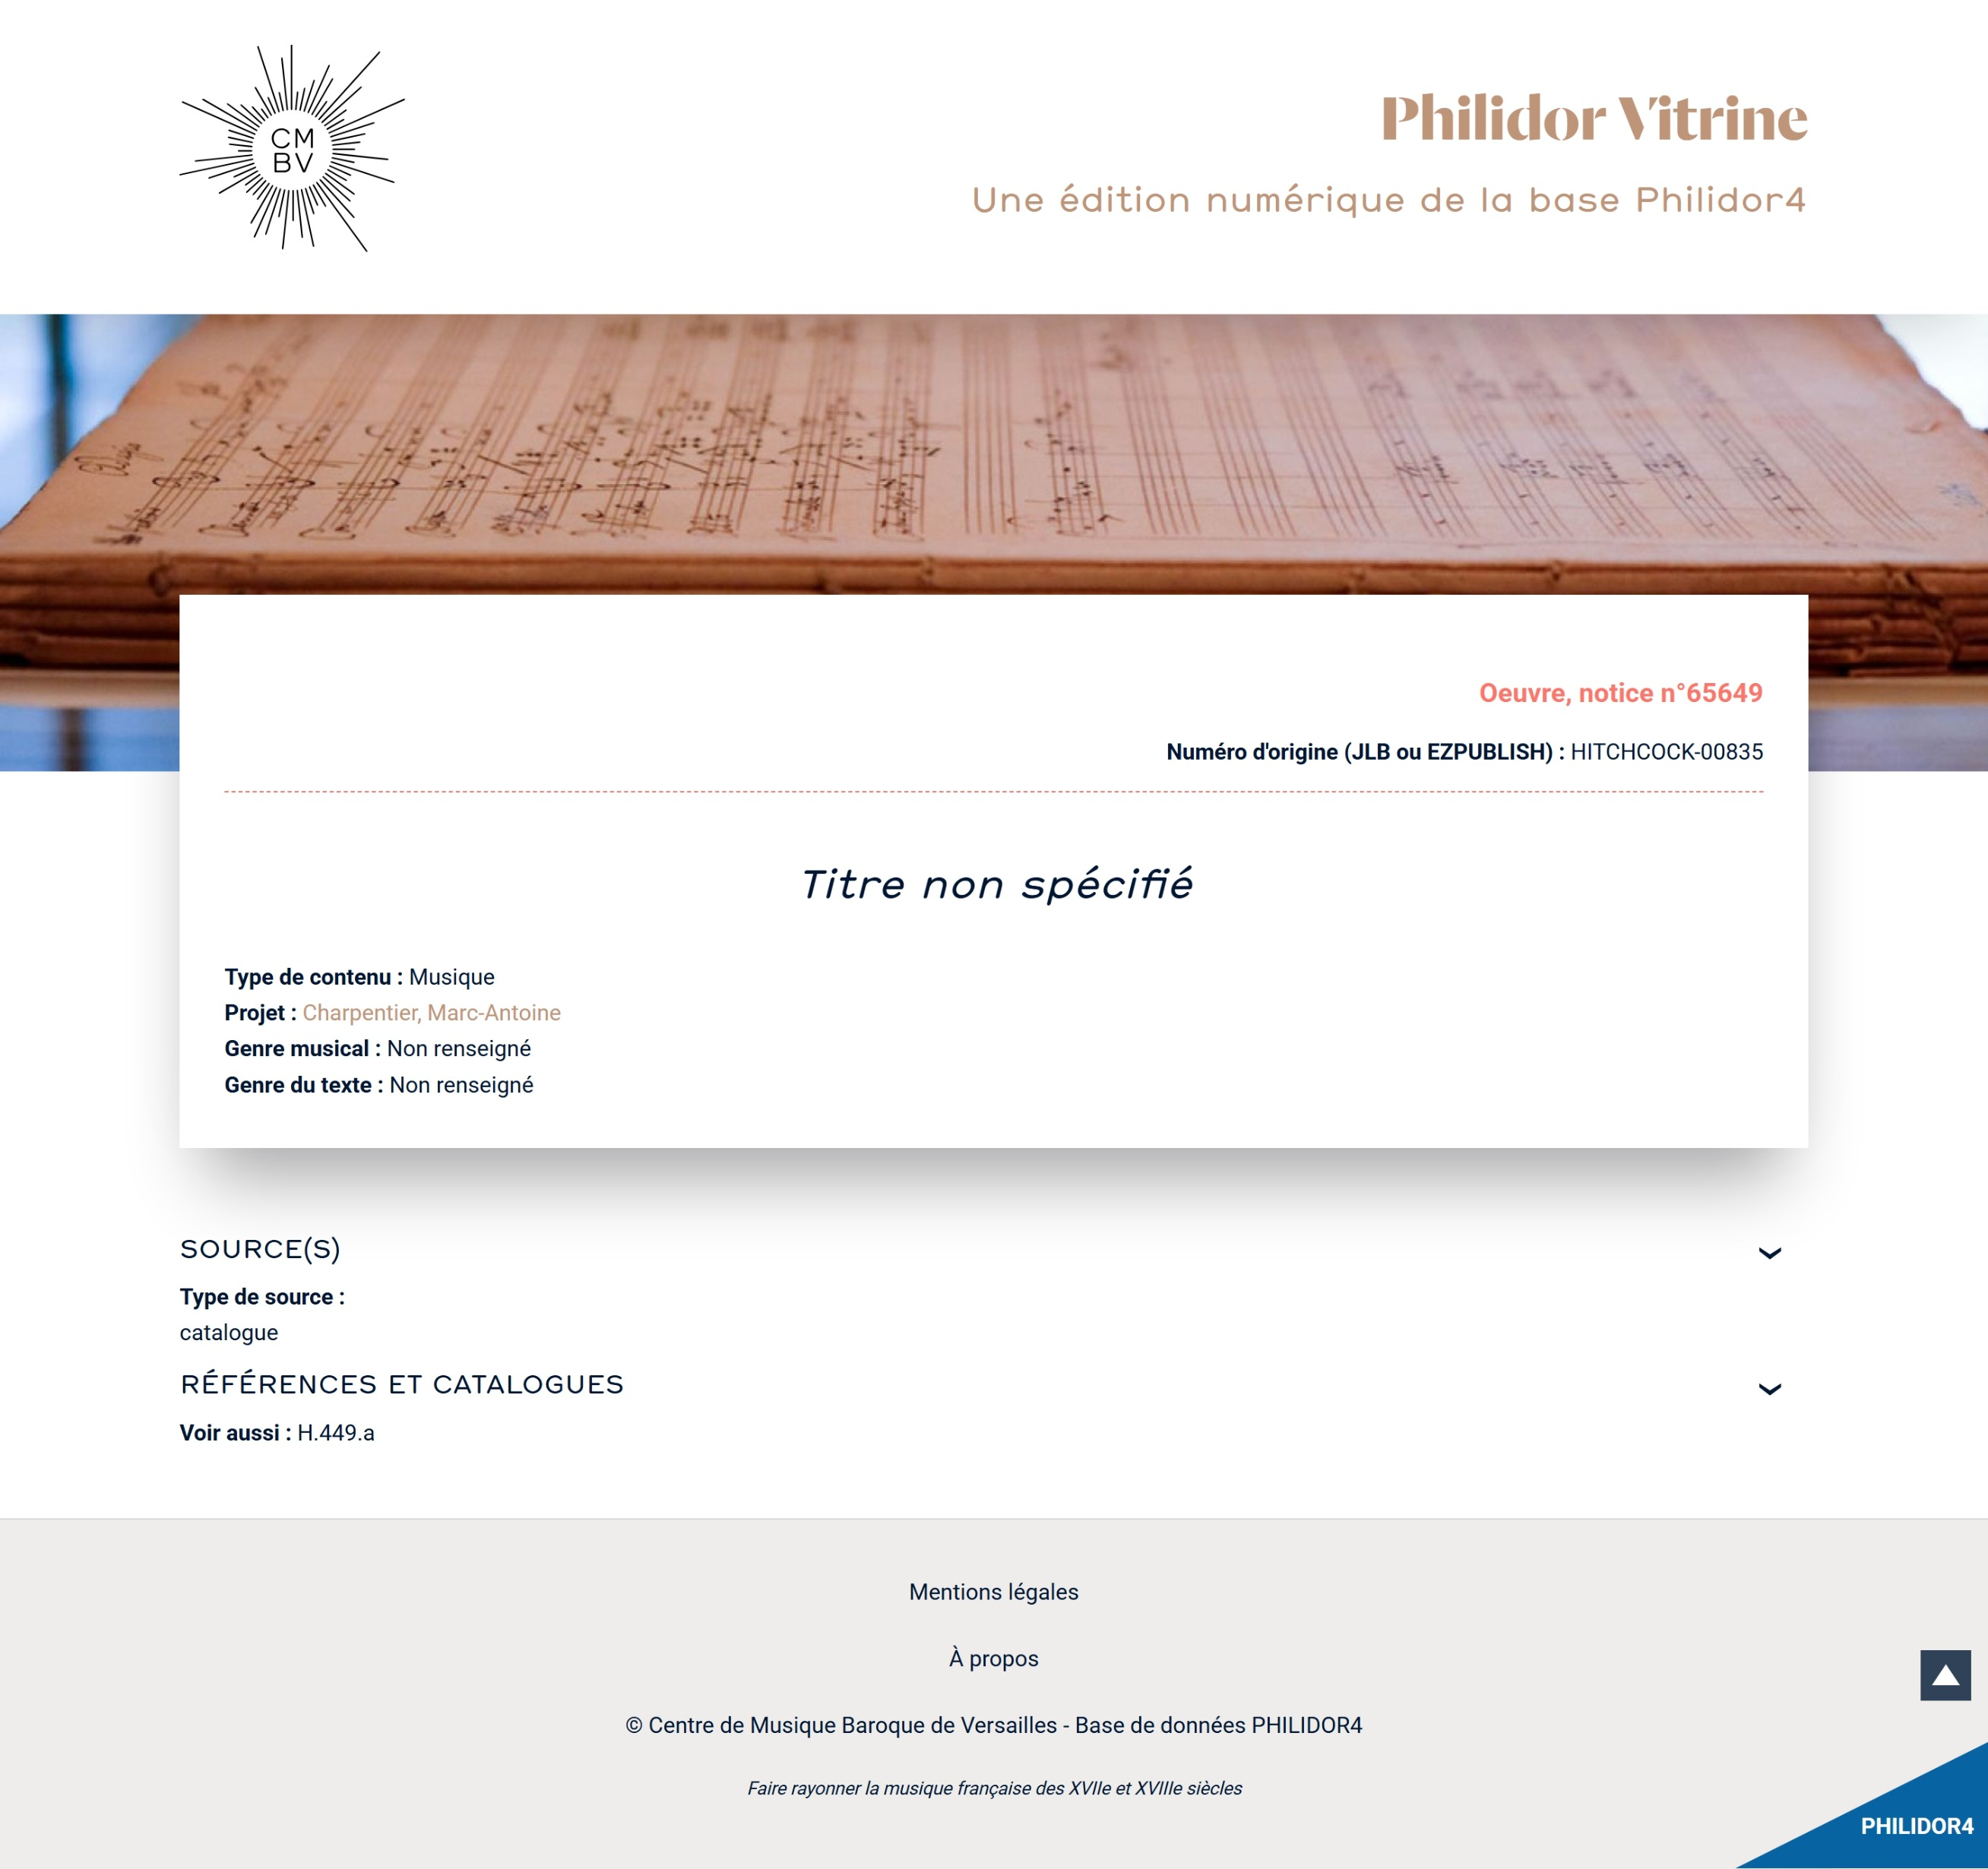
\includegraphics[width=\textwidth]{images/exemple-notice2-edition-philidor.jpeg}
\end{figure}

Cette approche de normalisation révèle les difficultés de passage entre logiques de catalogage savant et impératifs de lisibilité web.

\subsubsection{Solutions techniques adoptées et leurs limites}

Face à ces contraintes, plusieurs stratégies d'adaptation ont été développées. Le système de variables XPath et l'utilisation de clés permettent d'optimiser les performances malgré la complexité des recherches croisées. L'approche modulaire des templates facilite la maintenance et l'évolution du code de transformation.

Cependant, ces solutions techniques demeurent tributaires de la qualité des données sources. Les mécanismes d'indexation les plus sophistiqués ne peuvent compenser les lacunes documentaires originelles. La génération automatique atteint ainsi ses limites face à l'hétérogénéité irréductible des pratiques de catalogage historiques.

Le choix du format \gls{html} statique, s'il garantit la stabilité et l'accessibilité, limite également les possibilités d'enrichissement dynamique. L'absence de base de données côté client empêche l'implémentation de fonctionnalités de recherche avancée ou de visualisation interactive qui pourraient valoriser davantage la richesse des corpus.

\subsubsection{Perspectives d'évolution et positionnement stratégique}

L'avenir de l'édition web statique s'envisage selon plusieurs scénarios non exclusifs. L'enrichissement progressif constitue la voie la plus immédiate : l'outil d'édition et de génération Python développé permet d'intégrer de nouveaux projets et d'améliorer les descriptions contextuelles. Cette approche incrémentale pourrait transformer l'édition en véritable vitrine évolutive des activités de recherche du \gls{cmbv}.

L'adaptation de la feuille de style \gls{xslt} pourrait également étendre son champ d'application au-delà des seuls catalogues d'auteur. L'intégration de nouveaux types de projets (corpus thématiques, collections d'enregistrements, éditions critiques) nécessiterait des développements ciblés mais techniquement réalisables.

Un scénario alternatif envisage l'abandon de l'édition statique au profit d'améliorations directes de l'interface de \textit{Philidor~4}. Dans cette perspective, l'expérience web servirait d'exemple et d'inspiration pour moderniser l'outil principal. Les innovations développées (charte graphique cohérente, système d'accordéon, navigation hiérarchique) pourraient être intégrées dans une version renouvelée de la base de données.

Cette incertitude stratégique reflète un enjeu plus large : l'arbitrage entre outils spécialisés multiples et plateforme unifiée. L'édition web statique démontre la faisabilité technique d'une valorisation grand public des données musicologiques, mais questionne également la pertinence de multiplier les interfaces d'accès aux mêmes contenus.

L'expérience de construction de cette édition web, malgré ses limites techniques, ouvre ainsi des perspectives significatives pour la valorisation numérique des patrimoines musicologiques. Elle révèle les possibilités offertes par les technologies de transformation automatique tout en soulignant l'importance cruciale de la qualité des données sources et de la cohérence éditoriale d'ensemble.

\section*{Conclusion du chapitre}

L'expérimentation d'une \gls{editionwebstatique} appliquée aux données de \textit{Philidor~4} révèle la fécondité d'une approche éditoriale alternative aux interfaces de bases de données traditionnelles. En privilégiant la sélection raisonnée et la contextualisation narrative sur l'exhaustivité et la recherche libre, cette démarche ouvre des perspectives nouvelles pour la valorisation du patrimoine musical numérique.

L'analyse des fondements théoriques souligne la convergence entre les exigences scientifiques de l'éditorialisation musicologique et les avantages techniques de l'architecture statique. Les principes de contextualisation, essentiels à la compréhension de la musique baroque, trouvent dans cette approche un terrain d'application privilégié, tandis que les considérations de performance, de sécurité et de sobriété environnementale légitiment l'abandon des solutions dynamiques complexes. Cette convergence conceptuelle et technique dessine un modèle cohérent pour les institutions patrimoniales confrontées aux défis de la transition numérique.

La méthodologie développée, articulant outil Python collaboratif, sélection de corpus et architecture \gls{xslt}, démontre la faisabilité technique d'une automatisation éditoriale respectueuse des logiques scientifiques. Le corpus de quatorze projets, représentatif de la diversité des données de \textit{Philidor~4}, valide l'approche sur des cas concrets tout en révélant les adaptations nécessaires selon les types d'entités musicologiques. L'architecture de transformation confirme la pertinence des technologies standardisées pour la pérennité et la maintenabilité des dispositifs éditoriaux.

L'analyse technique de la construction du site web met en évidence les acquis et les limites de cette approche prototype. L'intégration réussie dans l'écosystème visuel du \gls{cmbv}, par la reprise cohérente des codes graphiques et des interactions, démontre la possibilité d'une appropriation institutionnelle harmonieuse. La navigation hiérarchique, respectueuse des logiques de consultation musicologique, facilite l'accès aux contenus tout en préservant leur organisation scientifique. Cependant, la complexité des relations entre œuvres, sources et fragments révèle les défis de l'automatisation de processus intellectuels sophistiqués. Si les solutions techniques développées permettent de reconstituer fonctionnellement ces liens, elles soulignent également les limites de la normalisation automatique face à l'hétérogénéité des données patrimoniales.

La gestion des données incomplètes ou erronées, bien que techniquement résolue par des mécanismes de récupération, pose des questions éditoriales fondamentales sur les critères de sélection et de présentation. Ces défis révèlent la tension persistante entre la richesse documentaire des corpus musicologiques et les impératifs de lisibilité des interfaces grand public.

Ce chapitre révèle ainsi l'ambivalence de l'édition numérique statique : solution prometteuse pour la valorisation éditoriale des données patrimoniales, elle demeure confrontée aux défis de la \glslink{mediationculturelle}{médiation} entre expertise scientifique et accessibilité publique. Le prototype développé constitue moins une solution définitive qu'un laboratoire méthodologique qui interroge les modalités contemporaines de transmission du patrimoine musical. Cette expérimentation ouvre sur une réflexion plus large concernant l'équilibre entre approches éditoriales et documentaires, entre automatisation technique et choix scientifiques, qui conditionne l'avenir des humanités numériques patrimoniales et leur capacité à concilier rigueur académique et démocratisation des savoirs.